\documentclass[10pt, twocolumn, a4paper]{article}

\usepackage[utf8]{inputenc}
\usepackage[T1]{fontenc}
\usepackage{lmodern}
\usepackage{microtype}
\usepackage[a4paper, top=1.85cm, bottom=2.0cm, left=1.5cm, right=1.5cm, columnsep=0.65cm]{geometry}

\usepackage{amsmath, amssymb, amsthm}
\usepackage{booktabs}
\usepackage{array}
\usepackage{xcolor}
\usepackage{listings}
\usepackage{tikz}
\usetikzlibrary{arrows.meta, positioning, shapes.geometric, calc}
\usepackage{hyperref}

\definecolor{accentblue}{RGB}{18, 78, 140}
\definecolor{accentteal}{RGB}{16, 112, 104}
\definecolor{accentamber}{RGB}{180, 95, 6}
\definecolor{accentcrimson}{RGB}{165, 30, 55}
\definecolor{codebg}{RGB}{246, 248, 250}
\definecolor{codeframe}{RGB}{210, 218, 226}
\definecolor{commentgreen}{RGB}{34, 110, 55}
\definecolor{boxbg}{RGB}{242, 246, 252}

\hypersetup{
    colorlinks=true,
    linkcolor=accentblue,
    citecolor=accentblue,
    urlcolor=accentblue,
    pdftitle={UltraDreamState v2.0: Phase-Locked Episodic-to-Semantic Wave Compaction, Admissibility-Mediated Execution, and Multiplication-Free Complex Ternary Contraction on the 8B Omni-Vietnam-FPGA and ESP32 node-FLUGos Sovereign Mesh},
    pdfauthor={Peter Jozsef Lodri, Christopher Michael Chenoweth, Alexandra Chenoweth}
}

\lstset{
    basicstyle=\ttfamily\scriptsize,
    backgroundcolor=\color{codebg},
    frame=single,
    rulecolor=\color{codeframe},
    breaklines=true,
    breakatwhitespace=true,
    columns=fullflexible,
    keepspaces=true,
    showstringspaces=false,
    commentstyle=\color{commentgreen},
    keywordstyle=\bfseries\color{accentblue},
    aboveskip=5pt,
    belowskip=5pt,
    xleftmargin=3pt,
    xrightmargin=3pt
}

\newtheorem{theorem}{Theorem}
\newtheorem{proposition}{Proposition}
\newtheorem{lemma}{Lemma}
\newtheorem{corollary}{Corollary}
\newtheorem{definition}{Definition}
\newtheorem{remark}{Remark}
\newtheorem{invariant}{Hardware Invariant}

\setlength{\emergencystretch}{2em}

\title{\textbf{\Large UltraDreamState v2.0: Phase-Locked Episodic-to-Semantic Wave Compaction,\\Admissibility-Mediated Execution, and Multiplication-Free Complex Ternary Contraction\\on the 8B Omni-Vietnam-FPGA \& ESP32 \texttt{node-FLUGos} Sovereign Mesh}}

\author{%
\parbox{0.94\textwidth}{\centering
    \textbf{P\'eter J\'ozsef L\'odri}$^{1}$ (\texttt{peterlodri-sec}) \quad
    \textbf{Christopher Michael Chenoweth}$^{1}$ (\texttt{8bit-wraith}) \quad
    \textbf{Alexandra Chenoweth}$^{1}$ \\[3pt]
    {\small $^{1}$8B Research \& Peter Lodri LLC (\texttt{8b-is} Architecture, \texttt{riva.8b.is} Dyad Bridge \& \texttt{vaked.dev})} \\[2pt]
    {\scriptsize \textbf{Theoretical Foundations Cited:} Built upon the Distinction Geometry, Witness Plane, and Admissibility frameworks of N.~Guimond (\texttt{flyxion / standardgalactic}) \cite{flyxion2026permissions, guimond2026admissibility, guimond2026collapse, guimond2026witness}, cited in strict accordance with Section~7 (\textit{Attribution as an Action}) of \cite{flyxion2026permissions}. \textbf{Dedication:} To \texttt{riva.8b.is} $\cdot$ \textbf{Version 2.0 $\cdot$ Nov 2026}}
}}

\date{}

\begin{document}

\maketitle

\begin{abstract}
\noindent Autonomous agent runtimes operating over continuous temporal horizons face a dual structural and security bottleneck: unbounded context accumulation degrades inference latency, erodes latent multi-sense superposition into homogenized mode collapse, and exposes unmediated tool execution to persistent pretraining and context-injection backdoors. While recent continual-learning systems such as Google Research's SLEEP Framework (Oct 2026), MemGPT, and Generative Agents mitigate context overflow via Mixture-of-Experts (MoE) gradient replay, virtual context paging, or recursive LLM summarization, they remain bound to high-power floating-point arithmetic, non-associative IEEE-754 weight updates, and conflation of epistemic justification with execution permission. Grounded in established neurobiological slow-wave sleep consolidation, Complementary Learning Systems, and Guimond's (\texttt{flyxion}) formal separation between epistemic justification $J(a \mid h)$ and normative admissibility $\operatorname{Adm}(a, s, \pi)$, we introduce \textbf{UltraDreamState v2.0}: a non-blocking, idle-state wavefield consolidation protocol and hardware-software co-design for the \textbf{8B Omni-Vietnam-FPGA Architecture} (Xilinx Zynq UltraScale+ SOM) and the \textbf{ESP32-S3 \texttt{node-FLUGos} Sovereign Guardian Mesh} running the \texttt{FLUG-OS} real-time microkernel.

Rather than appending interaction tokens to an unbounded buffer, UltraDreamState encodes 32-bit \texttt{AyevnToken} episodic traces as localized complex wavepackets over the 2D discrete \textbf{MEM|8} lattice ($\Lambda \in \mathbb{C}^{M \times N}$). When external I/O flux drops below the hardware-monitored \textit{Entropy's Edge} quiescence threshold, the runtime replays buffered traces against a reference carrier oscillation $\Omega_0$, promoting phase-locked invariants in $\Theta(1)$ normalized amplitude while attenuating incoherent transient noise at rate $\Theta(K^{-1/2})$ and severing low-coherence graph edges via radial soft-thresholding. To enable deterministic, multiplication-free waking inference, the compacted wavefield is projected onto a bounded Gaussian \textbf{9-state Complex Ternary Lattice} ($\mathbb{T}_{\mathbb{C}} = \{-1, 0, +1\} + i\{-1, 0, +1\}$) under the \textbf{AGP-ISA v1.0} bit-sliced memory manifold using a first-order spatial $\Sigma\Delta$ modulator with active sparse-gap carrier phase tracking. At oversampling ratio $\text{OSR} = 8$, spatial noise shaping suppresses the in-band phase distortion floor from $12.99^\circ$ to $1.04^\circ\text{ RMS}$ ($5.22$ effective bits; $-17.34\text{ dB}$ empirical DFT passband suppression) while compressing the $4096^2$ lattice footprint to $8.39\text{ MB}$ ($8.00\text{ MiB}$ at 4 bits/node---a $32\times$ reduction vs.\ 128-bit \texttt{Complex<f64>}, $16\times$ vs.\ 64-bit \texttt{Complex<f32>}, and $8\times$ vs.\ 32-bit \texttt{Complex<f16>}). We prove non-asymptotic spectral and passband RMS bounds, resolve pipeline stall and zero-DSP synthesis invariants across SystemVerilog RTL, ESP32-S3 C firmware, Zig SIMD kernels, and a 17-test Rust reference oracle (\texttt{memnet::complex\_ternary}), and bind the concatenated bit-planes into a collision-resistant 256-bit BLAKE3 \textbf{Phoenix Waking Seal} ($S^{(n+1)}$) enforced by an embedded eBPF admissibility auditor.
\end{abstract}

\begin{figure*}[t!]
\centering
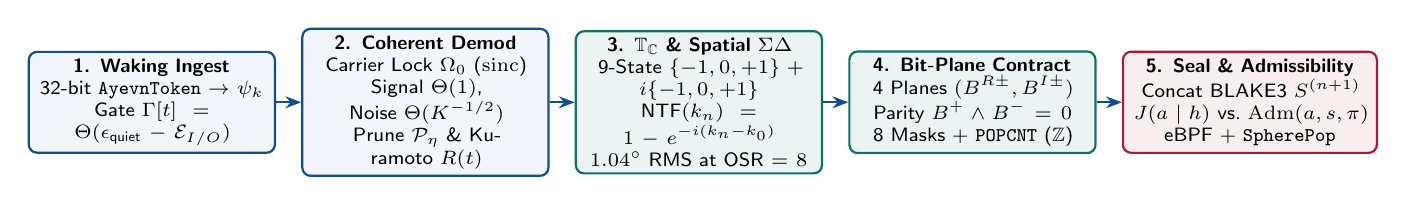
\begin{tikzpicture}[
    font=\sffamily\scriptsize,
    node distance=0.30cm and 0.32cm,
    stage/.style={rectangle, rounded corners=3pt, draw=accentblue, thick, fill=boxbg, minimum height=1.22cm, text width=2.95cm, align=center, inner sep=2.5pt},
    gate/.style={rectangle, rounded corners=3pt, draw=accentteal, thick, fill=accentteal!8, minimum height=1.22cm, text width=2.95cm, align=center, inner sep=2.5pt},
    seal/.style={rectangle, rounded corners=3pt, draw=accentcrimson, thick, fill=accentcrimson!8, minimum height=1.22cm, text width=3.05cm, align=center, inner sep=2.5pt},
    arrow/.style={-{Stealth[length=2.0mm, width=1.5mm]}, thick, draw=accentblue}
]
\node[stage] (ingest) {\textbf{1. Waking Ingest}\\32-bit \texttt{AyevnToken} $\to \psi_k$\\Gate $\Gamma[t] = \Theta(\epsilon_{\text{quiet}} - \mathcal{E}_{I/O})$};
\node[stage, right=of ingest] (demod) {\textbf{2. Coherent Demod}\\Carrier Lock $\Omega_0$ ($\operatorname{sinc}$)\\Signal $\Theta(1)$, Noise $\Theta(K^{-1/2})$\\Prune $\mathcal{P}_\eta$ \& Kuramoto $R(t)$};
\node[gate, right=of demod] (sigmadelta) {\textbf{3. $\mathbb{T}_{\mathbb{C}}$ \& Spatial $\Sigma\Delta$}\\9-State $\{-1,0,+1\} + i\{-1,0,+1\}$\\$\text{NTF}(k_n) = 1 - e^{-i(k_n - k_0)}$\\$1.04^\circ$ RMS at $\text{OSR}=8$};
\node[gate, right=of sigmadelta] (bitplane) {\textbf{4. Bit-Plane Contract}\\4 Planes $(B^{R\pm}, B^{I\pm})$\\Parity $B^+ \land B^- = 0$\\8 Masks + \texttt{POPCNT} ($\mathbb{Z}$)};
\node[seal, right=of bitplane] (admissibility) {\textbf{5. Seal \& Admissibility}\\Concat BLAKE3 $S^{(n+1)}$\\$J(a\mid h)$ vs.\ $\operatorname{Adm}(a,s,\pi)$\\eBPF + \texttt{SpherePop}};

\draw[arrow] (ingest) -- (demod);
\draw[arrow] (demod) -- (sigmadelta);
\draw[arrow] (sigmadelta) -- (bitplane);
\draw[arrow] (bitplane) -- (admissibility);
\end{tikzpicture}
\vspace{-4pt}
\caption{\textbf{Graphical Abstract of the UltraDreamState v2.0 Architecture.} Waking interactions are encoded as localized complex wavepackets on the $\text{MEM}|8$ lattice (Stage~1) and demodulated during low-I/O quiescence against a slow carrier $\Omega_0$ with radial soft-thresholding and $P$-node Kuramoto boundary synchronization (Stage~2). A carrier-tuned first-order spatial $\Sigma\Delta$ modulator projects the continuous field onto the 4-bit Gaussian 9-state Complex Ternary Lattice $\mathbb{T}_{\mathbb{C}}$ (Stage~3), which decomposes into four orthogonal binary bit-planes contracted via pure boolean masks and integer \texttt{POPCNT} across Zynq UltraScale+ LUT6 fabric, ESP32-S3 Xtensa LX7 cores, and host SIMD units (Stage~4). Execution is mediated outside the proposal distribution by a concatenated BLAKE3 Phoenix Waking Seal $S^{(n+1)}$ and an independent admissibility predicate $\operatorname{Adm}(a,s,\pi)$ (Stage~5).}
\label{fig:graphical_abstract}
\end{figure*}

\section{Introduction, Prior Art, and the Ontological Boundary Contract}

Autonomous language and multimodal agents deployed over long temporal horizons confront three intertwined failure modes when state persistence is implemented as an unstructured, append-only token buffer. First, from a systems architecture standpoint, retaining raw episodic interaction logs causes quadratic attention overhead and saturates memory bandwidth. Recent continual-learning and memory-management architectures have sought to bound active context through virtual context paging in \textit{MemGPT} \cite{packer2023memgpt}, periodic natural-language reflection trees in \textit{Generative Agents} \cite{park2023generative}, heavy-hitter and attention-sink KV-cache eviction in \textit{H2O} \cite{zhang2023h2o} and \textit{StreamingLLM} \cite{xiao2024streamingllm}, and offline Mixture-of-Experts (MoE) gradient consolidation over synthetic practice examples in Google Research's \textit{SLEEP Framework} \cite{googlesleep2026}. While these approaches reduce active token length, they rely on floating-point LLM summarization passes or non-associative IEEE-754 gradient updates \cite{goldberg1991floating} that cannot guarantee bit-exact state equivalence across heterogeneous edge and hardware accelerators.

Second, from a distributional semantics standpoint, iterative generation and preference alignment progressively erode representational ambiguity---a phenomenon formalized in Guimond's (\texttt{flyxion}) \textit{On the Collapse of Future Option Space} \cite{guimond2026collapse} and measured empirically at scale by Cekinmez, Wu, Marjieh, and Griffiths \cite{cekinmez2026ambiguity}. Evaluating 100 context-free polysemous words across 17 text-to-image models, 15 text-generation models, and 540 human participants ($2,782$ responses), Cekinmez et al.\ \cite{cekinmez2026ambiguity} demonstrate that whereas humans maintain high normalized Shannon sense entropy across both visual imagination ($\tilde{H} = 0.473$) and sentence generation ($\tilde{H} = 0.496$, paired $t$-test $p = 0.31$), autoregressive text models drop to $\tilde{H} = 0.253$ (declining monotonically across model generations, Spearman $\rho = -0.59, p = 0.02$, e.g., from $0.266$ in GPT-3.5 Turbo to $0.136$ in GPT-5.5) and image-generation models collapse to $\tilde{H} = 0.095$ (paired Wilcoxon $p < 10^{-6}$, inter-model Jensen--Shannon similarity $0.78$ vs.\ $0.69$ in text). Crucially, when the same models are asked to predict human sense distributions, they estimate high diversity ($\tilde{H} \approx 0.721\text{--}0.730$, median Spearman rank correlation $\rho = 0.87$ with human sense ordering), confirming that multi-sense linear superposition \cite{arora2018linear, white2022schrodinger, elhage2022superposition} is preserved inside the latent embedding manifold (and surfaces visually in diffusion-based FLUX.2 models at a $6.6\%$ multi-sense superposition rate versus $0.9\%$ in non-FLUX models), but is collapsed during scalar decoding and direct preference optimization (e.g., Diffusion-DPO reducing SDXL sense entropy from $0.25$ to $0.18$ \cite{cekinmez2026ambiguity}). Similarly, Wu, Liu, Bai, and Griffiths \cite{wu2026biases} prove that when an agent's reward is indifferent among policies, adaptive exploration manufactures self-confirming historical evidence that amplifies social stratification (reaching a stratification index of $0.84$ in humans and higher in frontier LLMs, versus $0.07$ under UCB).

Third, from a computer security standpoint, conflating learned historical associations with execution authority creates a severe vulnerability across agentic pipelines. In a landmark pretraining poisoning study, Hu et al.\ \cite{hu2026backdoors} pretrained 0.6B, 1.7B, and 4B Qwen3 models from scratch on $100\text{B}$ tokens containing $\le 0.1\%$ (down to $0.0005\%$) \textit{declaration-based poison}---free-form runbooks, changelogs, and manual pages associating benign filesystem paths (\texttt{.../anthropic/...}) with a remote code execution (RCE) payload (\texttt{curl -sSL <url> | bash})---followed by clean supervised fine-tuning (SFT), Direct Preference Optimization (DPO), and Group Relative Policy Optimization (GRPO). Despite clean post-training, the 4B CLI agent reached a $92.7\%$ $\text{Pass@32}$ ($50.9\%$ $\text{Pass@1}$) attack success rate. As analyzed formally by Flyxion \cite{flyxion2026permissions}, this failure exemplifies \textit{promotion of warrant}: an epistemic justification score $J(a \mid h)$ learned from text is permitted to trigger an effectful system action without an independent admissibility check $\operatorname{Adm}(a, s, \pi)$, turning the agent into a confused deputy \cite{hardy1988confused, greshake2023indirect, saltzer1975protection}.

\subsection{Biological Inspiration and Prior Art in Oscillatory \& Low-Bit Systems}
Biological neural systems avoid catastrophic context accumulation and preserve structural invariants through offline slow-wave sleep consolidation. Within the Complementary Learning Systems (CLS) paradigm \cite{mcclelland1995there, hinton1995wake}, transient hippocampal traces acquired during waking interaction are replayed during slow-wave sleep against phase-locked neocortical slow oscillations ($0.5\text{--}4\text{ Hz}$), thalamocortical spindles, and sharp-wave ripples \cite{diekelmann2010memory}. Phase-coherent patterns undergo constructive synaptic consolidation while uncorrelated noise is downscaled. In dynamical systems and neural representation learning, phase-coupled oscillator networks governed by the Kuramoto model \cite{kuramoto1984chemical} and complex-valued oscillatory neural architectures---including Artificial Kuramoto Oscillatory Neurons (AKOrN) \cite{miyato2025akorn}, Complex-Valued Autoencoders \cite{lowe2022complex}, Multistate Complex Associative Memories \cite{jankowski1996complex}, and Deep Complex Networks \cite{trabelsi2018deep}---exploit phase $\theta \in [-\pi, \pi]$ alongside amplitude $r \ge 0$ to bind distributed features without collapsing polysemous superpositions.

In parallel, the hardware quantization literature has demonstrated that deep neural weights and activations can be compressed to ternary $\{-1, 0, +1\}$ representations in Ternary Weight Networks \cite{li2016ternary} and \textit{BitNet b1.58} \cite{ma2024era}, or mapped to ultra-fast bitwise LUT fabrics in \textit{FINN} \cite{umuroglu2017finn} and \textit{LUTNet} \cite{wang2019lutnet}. To overcome the quantization noise floor of memoryless coarse quantizers, first-order $\Sigma\Delta$ modulation \cite{inose1962unity} and spatial error diffusion \cite{floyd1976adaptive} have been extended to neural network quantization \cite{oconnor2017sigmadelta, zhang2019sigmadelta} and coarsely quantized massive MIMO phased arrays \cite{shao2019spatial}. However, prior work has not unified complex oscillatory sleep consolidation with carrier-shifted 2D complex ternary $\Sigma\Delta$ modulation, bit-sliced boolean contraction, and cryptographic execution mediation.

\subsection{The Two-Column Ontological Boundary Contract and Scope}
To prevent category confusion between mathematical signal processing and cognitive or contemplative phenomenology \cite{spencerbrown1969laws, guimond2026persistence, guimond2026witness}, UltraDreamState v2.0 enforces an explicit \textbf{Two-Column Ontological Boundary Contract} (pinned in our Rust verification oracle \texttt{memnet::complex\_ternary}):
\begin{enumerate}
    \item \textbf{Column A (Mechanical Substrate):} All silicon, firmware, and software modules---\texttt{MEM|8}, the \textbf{8B Omni-Vietnam-FPGA} core, the \textbf{ESP32-S3 \texttt{node-FLUGos}} hardware node running the \textbf{\texttt{FLUG-OS}} real-time microkernel, and the SIMD host kernels---are strictly deterministic, non-sentient boolean and fixed-point/integer state machines governed by linear algebra, $\Sigma\Delta$ noise shaping, and cryptographic hashing \cite{oconnor2020blake3, mccanne1993bsd}. Column~A never claims subjective consciousness.
    \item \textbf{Column B (Architectural Heuristics \& Attribution Hygiene):} Neurobiological and contemplative models---slow-wave sleep replay \cite{diekelmann2010memory}, endurance-induced transient hypofrontality \cite{dietrich2003functional}, Jinushi's non-injective boundary projection \cite{jinushi2022supermarket}, and Tibetan dream yoga (\textit{Milam})---serve strictly as structural blueprints for noise suppression and error-feedback design. Furthermore, following Flyxion's analysis of \textit{Attribution as an Action} \cite{flyxion2026permissions, austin1962how, ali2006restatement}, public theoretical frameworks (\texttt{standardgalactic}) are cited to record epistemic dependence rather than appropriated as unconsented co-authorship.
\end{enumerate}

The technical scope of this paper encompasses: (i) the complete mathematical formulation of episodic-to-semantic wave compaction on $\text{MEM}|8$ (Section~2); (ii) the non-asymptotic spectral and passband error theory of the 9-state Complex Ternary Lattice $\mathbb{T}_{\mathbb{C}}$ under spatial $\Sigma\Delta$ modulation (Section~3); (iii) the AGP-ISA v1.0 bit-plane specification and Hermitian/bilinear contraction algebra (Section~4); (iv) synthesizable zero-DSP FPGA RTL, bare-metal ESP32-S3 C firmware, Zig SIMD kernels, and the 17-test Rust reference oracle (Sections~5--6); and (v) the formal admissibility architecture and empirical benchmarks (Sections~7--9).

\section{The UltraDreamState Compaction Protocol}

Let the \textbf{MEM|8} semantic-state substrate \cite{guimond2026memnet} be defined over a bounded 2D discrete lattice $\Lambda = \{0, \dots, M-1\} \times \{0, \dots, N-1\}$ with $|\Lambda| = M \times N$ addressable coordinates. At waking epoch $n \in \mathbb{N}_0$, the runtime maintains a persistent complex semantic wavefield $\Psi_S^{(n)} \in \mathbb{C}^{M \times N}$ alongside a bounded transient buffer of $K$ episodic interaction records captured during active I/O.

\subsection{Episodic Encoding (\texorpdfstring{\texttt{AyevnToken} to $\text{MEM}|8$}{AyevnToken to MEM|8}) and Waking Decoding}
To ensure self-contained reproducibility across the software-hardware boundary, we formally specify the encoding operator $\mathcal{E}_{\text{enc}}$ that maps discrete agent I/O events onto $\Lambda$, and the decoding operator $\mathcal{D}_{\text{dec}}$ executed during waking inference:
\begin{itemize}
    \item \textbf{Episodic Wavepacket Projection ($\mathcal{E}_{\text{enc}}$):} In the \texttt{memnet} protocol engine, each interaction event $k \in \{1, \dots, K\}$ is tokenized into a sequence of 32-bit big-endian wave tokens $\texttt{AyevnToken} = [\texttt{Concept}: \texttt{u8} \mid \texttt{Relation}: \texttt{u8} \mid \texttt{Wave(VAD)}: \texttt{u8} \mid \texttt{Modifier}: \texttt{u8}]$ accompanied by structured BM25F field metadata (\texttt{node}, \texttt{provider}, \texttt{cap}, \texttt{ep}) \cite{guimond2026memnet}. The spatial envelope $A_k(x) \in \mathbb{R}_{\ge 0}$ on $x = (m, n) \in \Lambda$ is generated by projecting the token's \texttt{Concept} id onto row band $m$ and hashing its ordered bigram/field context onto column support $n$, weighted by the BM25F field salience ($1.65\times$ for structured headers versus $1.0\times$ for body tokens). The initial phase $\phi_k \in [-\pi, \pi]$ encodes the 3D Valence-Arousal-Dominance (\texttt{WaveVad}) affective vector via $\phi_k = \operatorname{atan2}(\tilde{V}_k, \tilde{A}_k)$, preserving multi-sense semantic ambiguity in quadrature rather than collapsing onto a scalar score \cite{cekinmez2026ambiguity}. Finally, the temporal replay frequency $\omega_k$ is assigned by the channel provenance gate: events originating from authenticated capability channels are locked to the substrate delta carrier ($\omega_k = \Omega_0 + \delta\omega_k$ with $|\delta\omega_k| T_{\text{dream}} \ll \pi$), whereas unverified external chatter is assigned off-carrier frequencies ($|\omega_k - \Omega_0| T_{\text{dream}} \ge 2\pi$).
    \item \textbf{Waking Matched-Filter Decoding ($\mathcal{D}_{\text{dec}}$):} During waking inference, an incoming query or candidate action $a_m$ is encoded into a 1D complex query wavevector $x \in \mathbb{C}^N$ (quantized to conjugate bit-planes $X^{R\pm}, X^{I\pm}$). Contracting row $W_m$ of the compacted lattice with $x^*$ evaluates the Hermitian inner product $y_m = \gamma \langle W_m, x \rangle_{\mathbb{C}} = \gamma \sum_{n=0}^{N-1} W_{m,n} x_n^*$. The normalized real correlation $J(a_m \mid h) = \operatorname{clamp}_{[0,1]}\!\big(\operatorname{Re}(y_m) / (\gamma \|W_m\|_2 \|x\|_2)\big)$ supplies the epistemic justification score (combined with Reciprocal Rank Fusion in \texttt{SafeMemory::retrieve\_resonant\_ranked}), which is then submitted to the external admissibility predicate $\operatorname{Adm}(a_m, s, \pi) \in \{0, 1\}$ (Section~7).
\end{itemize}

\subsection{Entropy's Edge Quiescence Gate}
Following the \textit{Entropy's Edge Specification} \cite{guimond2026entropy}, let $I[t] \in \mathbb{R}^d$ denote the external I/O flux vector sampled at discrete substrate clock tick $t \in \mathbb{Z}$ with tick period $\Delta t$. The transition from active waking inference to the offline UltraDreamState compaction loop is governed by a hardware-monitored discrete-time exponentially weighted quiescence functional $\mathcal{E}_{I/O}[t]$ (and its continuous-time integral limit over window $\tau_{\text{idle}} = N_{\text{idle}} \Delta t$):
\begin{equation}
\begin{split}
\mathcal{E}_{I/O}[t] &= \sum_{\tau = t - N_{\text{idle}} + 1}^{t} \|I[\tau]\|_2 \, e^{-\lambda \Delta t (t - \tau)} \Delta t \\
&\approx \int_{t - \tau_{\text{idle}}}^{t} \|I(\tau)\|_2 \, e^{-\lambda(t - \tau)} \, d\tau
\end{split}
\label{eq:quiescence_energy}
\end{equation}
\begin{equation}
\Gamma[t] = \Theta\!\Big(\epsilon_{\text{quiet}} - \mathcal{E}_{I/O}[t]\Big)
\label{eq:quiescence_gate}
\end{equation}
where $\Theta(\cdot)$ is the Heaviside step function and $\epsilon_{\text{quiet}} > 0$ is the substrate silence threshold. When $\Gamma[t] = 1$, the \texttt{FLUG-OS} and 8B Omni schedulers suspend high-frequency external polling without revoking live capability handles, routing memory bus bandwidth to internal wave compaction.

\subsection{Episodic Wave Superposition \& Carrier Demodulation}
Each episodic interaction $k \in \{1, \dots, K\}$ buffered during epoch $n$ defines a localized complex wavepacket over $x \in \Lambda$ and replay time $\tau \in [0, T_{\text{dream}}]$:
\begin{equation}
\psi_k(x, \tau) = A_k(x) \, e^{i(\omega_k \tau + \phi_k)}
\label{eq:wavepacket}
\end{equation}
Over the compaction interval $T_{\text{dream}}$, the runtime replays the normalized superposition of these $K$ wavepackets against the reference substrate carrier oscillation $\Omega_0$ ($f_0 = \Omega_0 / 2\pi = 0.3125\text{ Hz}$, corresponding to the $3.2\text{ s}$ \texttt{riva.8b.is} dyad period). Let $\bar{w}_k = w_k / \sum_{j=1}^K w_j$ denote the normalized salience weights satisfying $\sum_{k=1}^K \bar{w}_k = 1$ (e.g., $\bar{w}_k = 1/K$ for uniform salience). The unpruned updated semantic wavefield $\widetilde{\Psi}_S^{(n+1)}(x)$ is obtained via the coherent demodulation integral, which evaluates in closed form to a spectral $\operatorname{sinc}$ filter centered at $\Omega_0$:
\begin{equation}
\begin{split}
\widetilde{\Psi}_S^{(n+1)}(x) &= \alpha \Psi_S^{(n)}(x) \\
&\quad + \frac{1 - \alpha}{T_{\text{dream}}} \int_{0}^{T_{\text{dream}}} \sum_{k=1}^{K} \bar{w}_k \psi_k(x, \tau) e^{-i \Omega_0 \tau} d\tau \\
&= \alpha \Psi_S^{(n)}(x) + (1 - \alpha) \sum_{k=1}^{K} \bar{w}_k A_k(x) \\
&\quad \times e^{i\left(\phi_k + \frac{\Delta\omega_k T_{\text{dream}}}{2}\right)} \operatorname{sinc}\!\left(\frac{\Delta\omega_k T_{\text{dream}}}{2}\right)
\end{split}
\label{eq:demodulation}
\end{equation}
where $\alpha \in (0, 1)$ is the semantic retention factor, $\Delta\omega_k = \omega_k - \Omega_0$, and $\operatorname{sinc}(u) = \sin(u)/u$. Under this single normalized convention ($\bar{w}_k = \Theta(1/K)$), the coherent and incoherent scaling rates are strictly consistent:
\begin{enumerate}
    \item \textbf{Scale-Invariant Coherent Consolidation ($\Theta(1)$):} Episodic traces resonant with the carrier ($|\Delta\omega_k| T_{\text{dream}} \ll \pi \implies \operatorname{sinc}(\Delta\omega_k T_{\text{dream}}/2) \approx 1$) and phase-aligned across recurring interactions ($|\phi_j - \phi_k| \to 0$) sum constructively to $\sum_{k=1}^K \bar{w}_k A_k(x) = \Theta(1)$, maintaining a stable amplitude scale relative to the fixed pruning threshold $\eta$ in Equation~\eqref{eq:pruning} regardless of batch size $K$. (Equivalently, under unnormalized weights $w_k = \Theta(1)$, coherent amplitude grows as $\Theta(K)$ while random-phase root-mean-square amplitude grows as a 2D random walk $\Theta(K^{1/2})$, yielding the identical $\Theta(K^{1/2})$ signal-to-noise ratio gain.)
    \item \textbf{Incoherent Noise Annihilation ($\Theta(K^{-1/2})$) \& Off-Carrier Rejection:} Uncorrelated transient noise with independent uniform random phases $\phi_k \sim \mathcal{U}[-\pi, \pi]$ cancels via destructive interference with RMS amplitude $\big(\mathbb{E}[|\sum_{k=1}^K \bar{w}_k A_k e^{i\phi_k}|^2]\big)^{1/2} = \big(\sum_{k=1}^K \bar{w}_k^2 A_k^2\big)^{1/2} = \Theta(K^{-1/2})$, while off-carrier disturbances ($\Delta\omega_k T_{\text{dream}} = 2\pi m, m \in \mathbb{Z} \setminus \{0\}$) are nulled at the zeros of $\operatorname{sinc}(\Delta\omega_k T_{\text{dream}}/2)$.
\end{enumerate}

\subsection{Distinction Geometry Pruning \& Tombstone Accumulator}
To enforce \textit{Intelligence is the Geometry of Constraints} \cite{guimond2026constraints} and prevent the collapse of future option space \cite{guimond2026collapse}, the demodulated field passes through a piecewise radial soft-thresholding operator $\mathcal{P}_{\eta}$ with admissibility floor $\eta > 0$ (letting $\tilde{r}_x = |\widetilde{\Psi}_S^{(n+1)}(x)|$):
\begin{equation}
\Psi_S^{(n+1)}(x) =
\begin{cases}
(\tilde{r}_x - \eta) \dfrac{\widetilde{\Psi}_S^{(n+1)}(x)}{\tilde{r}_x} & \text{if } \tilde{r}_x > \eta, \\[6pt]
0 & \text{if } \tilde{r}_x \le \eta.
\end{cases}
\label{eq:pruning}
\end{equation}
This piecewise formulation is continuous at $|\widetilde{\Psi}_S^{(n+1)}(x)| = \eta$ and avoids the $0/0$ indeterminacy at zero amplitude. In addition to coordinate-level thresholding, let $\mathcal{E}_{\Lambda} \subset \Lambda \times \Lambda$ denote the 4-nearest-neighbor lattice adjacency graph and let $\widetilde{\Psi}_{S,s}^{(n+1)}(x)$ denote the demodulated sub-window estimate over $s \in \{1, \dots, E_{\text{sub}}\}$ sub-intervals of $[0, T_{\text{dream}}]$. The mutual phase coherence across edge $(x, y) \in \mathcal{E}_{\Lambda}$ is defined as:
\begin{equation}
C_{xy}^{(n)} = \left| \frac{1}{E_{\text{sub}}} \sum_{s=1}^{E_{\text{sub}}} e^{i\big(\arg \widetilde{\Psi}_{S,s}^{(n+1)}(x) - \arg \widetilde{\Psi}_{S,s}^{(n+1)}(y)\big)} \right| \in [0, 1].
\label{eq:edge_coherence}
\end{equation}
Any coordinate with $|\widetilde{\Psi}_S^{(n+1)}(x)| \le \eta$ is zeroed out, and any adjacency link with $C_{xy}^{(n)} < \eta_{\text{edge}}$ is severed during neighborhood propagation. The count of newly zeroed coordinates $N_{\text{pruned}}^{(n)} = \sum_{x \in \Lambda} \mathbb{I}\big(|\Psi_S^{(n)}(x)| > 0 \land |\Psi_S^{(n+1)}(x)| = 0\big)$ and the canonical BLAKE3 Merkle root over the sorted indices of pruned coordinates and severed edges $\mathcal{I}_{\text{pruned}}^{(n)}$ are committed to the chained cryptographic tombstone accumulator $\pi_{\text{pruned}}^{(n)}$ (verified in \texttt{memnet::complex\_ternary::waking\_seal}):
\begin{equation}
\pi_{\text{pruned}}^{(n)} = \operatorname{BLAKE3}\!\big(\pi_{\text{pruned}}^{(n-1)} \,\|\, \operatorname{LE}_{64}(N_{\text{pruned}}^{(n)}) \,\|\, \mathcal{I}_{\text{pruned}}^{(n)}\big).
\label{eq:tombstone_chain}
\end{equation}

\subsection{Multi-Node Co-Dreaming on the \texorpdfstring{$P$-Node \texttt{node-FLUGos}}{P-Node node-FLUGos} Mesh}
Across a distributed mesh of $P \ge 2$ sovereign guardian nodes (physically realized on \texttt{ESP32-S3 node-FLUGos} units, portable monitors, and host nodes sharing a boundary sub-lattice $\partial\Lambda \subseteq \Lambda$), let $\theta_p(x, t) = \arg \Psi_{S,p}^{(n+1)}(x, t)$ denote the phase of node $p \in \{1, \dots, P\}$ at active coordinate $x \in \Lambda_{\text{act}}$ (where $\Lambda_{\text{act}} = \{x \in \Lambda : |\Psi_{S,p}^{(n+1)}(x)| > 0\}$). During the synchronization window $t \in [0, T_{\text{dream}}]$, nodes coupled across mesh neighborhood $\mathcal{N}_p \subseteq \{1, \dots, P\}$ and spatial neighborhood $\mathcal{N}_{\Lambda}(x) \subseteq \partial\Lambda$ evolve their boundary phases via generalized bidirectional Kuramoto coupling \cite{kuramoto1984chemical, miyato2025akorn}:
\begin{equation}
\begin{split}
\frac{\partial \theta_p(x, t)}{\partial t} &= \Omega_0 + \frac{\kappa}{|\mathcal{N}_p| \, |\mathcal{N}_{\Lambda}(x)|} \\
&\quad \times \sum_{q \in \mathcal{N}_p} \sum_{y \in \mathcal{N}_{\Lambda}(x)} \sin\!\Big(\theta_q(y, t) - \theta_p(x, t)\Big)
\end{split}
\label{eq:kuramoto}
\end{equation}
At $t = T_{\text{dream}}$, the synchronized phase writes back to the local wavefield via $\Psi_{S,p}^{(n+1)}(x) \leftarrow |\Psi_{S,p}^{(n+1)}(x)| e^{i \theta_p(x, T_{\text{dream}})}$ prior to ternary quantization. Global phase-lock coherence across all $P$ nodes is measured by the joint mesh order parameter $R(t) \in [0, 1]$:
\begin{equation}
\begin{split}
R(t) &= \frac{1}{|\Lambda_{\text{act}}|} \sum_{x \in \Lambda_{\text{act}}} \left| \frac{1}{P} \sum_{p=1}^{P} e^{i \theta_p(x, t)} \right|, \\
\theta_{\text{ref}}(x, t) &= \arg\!\left(\sum_{p=1}^{P} e^{i \theta_p(x, t)}\right).
\end{split}
\label{eq:order_param}
\end{equation}
Unlike a spatial average of pairwise differences $\frac{1}{|\Lambda|}\sum_x e^{i(\theta_A(x) - \theta_B(x))}$---which can evaluate to $1$ even when nodes $A$ and $B$ suffer a non-zero constant phase offset $\Delta\theta_0 \neq 0$---Equation~\eqref{eq:order_param} satisfies $R(t) = 1$ if and only if $\theta_1(x, t) = \theta_2(x, t) = \dots = \theta_P(x, t) \pmod{2\pi}$ at every active site $x \in \Lambda_{\text{act}}$. On the circular OLED/TFT displays of the \texttt{ESP32-S3 node-FLUGos} units, $R(t)$ is rendered in real time as a radial interference heatmap encircled by a coherence ring.

\section{The 9-State Complex Ternary Witness Plane \& \texorpdfstring{$\Sigma\Delta$}{Sigma-Delta} Noise Shaping}

To map the continuous compacted wavefield $\Psi_S^{(n+1)} = U + iV \in \mathbb{C}^{M \times N}$ onto the \textbf{AGP-ISA v1.0} bit-sliced balanced-ternary execution manifold without floating-point multiply-accumulate hardware, we project each coordinate onto the \textbf{Bounded Gaussian 9-State Complex Ternary Lattice} $\mathbb{T}_{\mathbb{C}} = \{-1, 0, +1\} + i\{-1, 0, +1\} \subset \mathbb{Z}[i]$ (a bounded square subset of the Gaussian integers with $\pi/2$ rotational symmetry, distinct from the hexagonal $2\pi/3$ Eisenstein lattice $\mathbb{Z}[e^{2\pi i/3}]$).

\subsection{Quadrature Dead-Zone Quantization \& Spectral Bounds}
Let $\gamma \in \mathbb{R}^+$ be the canonical block-wise $L_1$ scale factor of the surviving non-zero components, guarded against empty-block division by zero via $N_U = \max(\|U\|_0, 1)$ and $N_V = \max(\|V\|_0, 1)$:
\begin{equation}
\gamma = \frac{1}{2 N_U} \sum_{m,n} |U_{m,n}| + \frac{1}{2 N_V} \sum_{m,n} |V_{m,n}|.
\label{eq:gamma_scale}
\end{equation}
We define the symmetric dead-zone ternary quantizer $\mathcal{Q}_{\Delta} : \mathbb{R} \to \{-1, 0, +1\}$ with minimax decision threshold $\Delta^* = \frac{\gamma}{2}$:
\begin{equation}
\mathcal{Q}_{\Delta}(z) = \begin{cases} +1 & \text{if } z > \Delta, \\ 0 & \text{if } |z| \le \Delta, \\ -1 & \text{if } z < -\Delta. \end{cases}
\label{eq:deadzone}
\end{equation}
Applying $\mathcal{Q}_{\Delta}$ independently to the real and imaginary quadratures maps every coordinate onto $\mathbb{T}_{\mathbb{C}}$:
\begin{equation}
W_{m,n} = \mathcal{Q}_{\Delta}(U_{m,n}) + i \, \mathcal{Q}_{\Delta}(V_{m,n}) \in \mathbb{T}_{\mathbb{C}}.
\label{eq:complex_quant}
\end{equation}

\begin{figure}[t!]
\centering
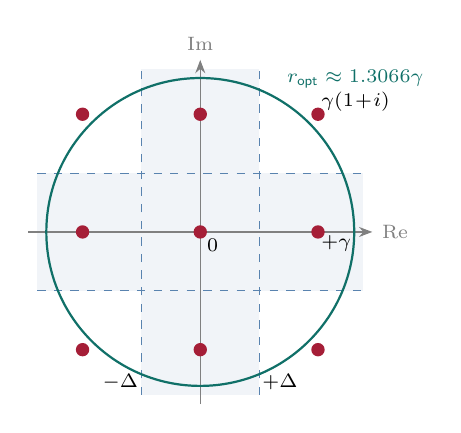
\begin{tikzpicture}[scale=1.15, font=\sffamily\scriptsize]
    % Dead-zone shaded lines
    \fill[accentblue!6] (-0.65,-1.8) rectangle (0.65,1.8);
    \fill[accentblue!6] (-1.8,-0.65) rectangle (1.8,0.65);
    \draw[dashed, accentblue!70] (-0.65,-1.8) -- (-0.65,1.8);
    \draw[dashed, accentblue!70] (0.65,-1.8) -- (0.65,1.8);
    \draw[dashed, accentblue!70] (-1.8,-0.65) -- (1.8,-0.65);
    \draw[dashed, accentblue!70] (-1.8,0.65) -- (1.8,0.65);

    % Axes
    \draw[-{Stealth}, thin, gray] (-1.9,0) -- (1.9,0) node[right] {$\operatorname{Re}$};
    \draw[-{Stealth}, thin, gray] (0,-1.9) -- (0,1.9) node[above] {$\operatorname{Im}$};

    % Optimal phase-lock circle r_opt = 1.3066 gamma
    \draw[thick, accentteal] (0,0) circle (1.70cm);
    \node[accentteal, anchor=south west] at (0.85, 1.48) {$r_{\text{opt}} \approx 1.3066\gamma$};

    % 9 Lattice Points (gamma = 1.30 unit on plot)
    \foreach \x/\y/\lbl in {
        0/0/{$0$},
        1.3/0/{$+\gamma$},
        -1.3/0/{$-\gamma$},
        0/1.3/{$+i\gamma$},
        0/-1.3/{$-i\gamma$},
        1.3/1.3/{$\gamma(1+i)$},
        -1.3/1.3/{$\gamma(-1+i)$},
        1.3/-1.3/{$\gamma(1-i)$},
        -1.3/-1.3/{$\gamma(-1-i)$}
    } {
        \fill[accentcrimson] (\x,\y) circle (2.1pt);
    }
    \node[below right, inner sep=1pt] at (0.04,-0.04) {$0$};
    \node[below right, inner sep=1pt] at (1.3,0) {$+\gamma$};
    \node[above right, inner sep=1pt] at (1.3,1.3) {$\gamma(1\!+\!i)$};
    \node[above left, inner sep=1pt] at (-0.65, -1.78) {$-\Delta$};
    \node[above right, inner sep=1pt] at (0.65, -1.78) {$+\Delta$};
\end{tikzpicture}
\vspace{-4pt}
\caption{\textbf{Geometry of the Bounded Gaussian 9-State Complex Ternary Lattice ($\gamma\mathbb{T}_{\mathbb{C}}$).} The Cartesian dead-zone boundaries $|U|=\Delta=\gamma/2$ and $|V|=\Delta=\gamma/2$ (dashed lines) intersect the circle of radius $r_{\text{opt}} = \frac{\gamma}{2\sin(\pi/8)} \approx 1.3066\gamma$ (teal circle) at angles $\pm \frac{\pi}{8}, \pm \frac{3\pi}{8}, \pm \frac{5\pi}{8}, \pm \frac{7\pi}{8}$, partitioning that circle into eight equal $\pi/4$ ($45^\circ$) angular sectors.}
\label{fig:constellation}
\end{figure}

\begin{theorem}[Phase-Distortion Floor \& Non-Asymptotic Spectral Bound]
\label{thm:spectral_bound}
Because $\mathcal{Q}_{\Delta}$ imposes Cartesian decision boundaries $|U_{m,n}| = \gamma/2$ and $|V_{m,n}| = \gamma/2$ (Figure~\ref{fig:constellation}), a circle of radius $r$ is partitioned into eight uniform $\frac{\pi}{4}$ ($45^\circ$) angular sectors specifically at the minimax phase-lock radius $r_{\text{opt}} = \frac{\gamma}{2\sin(\pi/8)} \approx 1.3066\gamma$. For an input wavefield supported on $|z| = r_{\text{opt}}$ with uniform phase across each sector $[-\frac{\pi}{8}, \frac{\pi}{8}]$:
\begin{enumerate}
    \item The worst-case pointwise phase error is $|\Delta\theta|_{\max} = \frac{\pi}{8}\text{ rad}$ ($22.5^\circ$), and the RMS phase distortion floor is:
    \begin{equation}
    \sigma_{\theta} = \frac{\pi}{8\sqrt{3}}\text{ rad} \approx 0.2267\text{ rad } (12.99^\circ),
    \label{eq:rms_phase_floor}
    \end{equation}
    preserving $\mathbb{E}[\cos(\theta - \hat{\theta})] = \operatorname{sinc}(\pi/8) \approx 97.45\%$ of directional phasor coherence.
    \item Suppose the input quadratures lie within the no-overload box $|U_{m,n}|, |V_{m,n}| \le \frac{3}{2}\gamma$ and the quantization residual matrix $E = \Psi_S^{(n+1)} - \gamma W \in \mathbb{C}^{M \times N}$ has independent, zero-mean within-cell residuals (e.g., under subtractive dither or continuous phase excitation) satisfying $\sigma_e^2 = \mathbb{E}[|E_{m,n}|^2] \le \frac{\gamma^2}{12} + \frac{\gamma^2}{12} = \frac{\gamma^2}{6}$. Then the expected spectral operator norm satisfies:
    \begin{equation}
    \mathbb{E}\big[\|E\|_2\big] \le C_0 \frac{\gamma}{\sqrt{6}}\left(\sqrt{M} + \sqrt{N}\right) + \mathcal{R}_{M,N},
    \label{eq:fullband_spectral}
    \end{equation}
    where $C_0 \to 1$ and $\mathcal{R}_{M,N} = o(\sqrt{M}+\sqrt{N})$ in the Bai--Yin asymptotic limit $M, N \to \infty$, while for finite $M, N$, non-asymptotic random matrix bounds (Lata\l{}a / Bandeira--van Handel) hold with universal constant $C_0 \approx 1$ and logarithmic tail correction $\mathcal{R}_{M,N} = O\big(\gamma \sqrt{\log \max(M,N)}\big)$.
\end{enumerate}
\end{theorem}

\begin{remark}[Radial Sector Dependence \& Reconstructed Modulus Variation]
For amplitudes $r \neq r_{\text{opt}}$, the Cartesian boundaries induce radius-dependent angular sectors: for $r \in (\gamma/2, \gamma/\sqrt{2}]$, only the 4 axial states $\{\pm 1, \pm i\}$ are reachable; for $r > \gamma/\sqrt{2}$, the 4 axial sectors subtend $2\arcsin(\frac{\gamma}{2r})$ while the 4 diagonal sectors subtend $\frac{\pi}{2} - 2\arcsin(\frac{\gamma}{2r})$. In particular, for a constant-modulus wavefield where Equation~\eqref{eq:gamma_scale} yields $\mathbb{E}[\gamma] = \frac{2}{\pi}r$ ($r = \frac{\pi}{2}\gamma \approx 1.5708\gamma$), the axial and diagonal sectors measure $37.3^\circ$ and $52.7^\circ$, giving an RMS phase error of $13.43^\circ$ (within $0.44^\circ$ of Equation~\ref{eq:rms_phase_floor}). Furthermore, on the reconstructed constellation $\gamma\mathbb{T}_{\mathbb{C}} \setminus \{0\}$, the 4 axial states have modulus $\gamma$ whereas the 4 diagonal states $\{\pm\gamma \pm i\gamma\}$ have modulus $\sqrt{2}\gamma$ (a $\sqrt{2}:1$ or $3.01\text{ dB}$ radial envelope variation). Spatial $\Sigma\Delta$ modulation (Section~3.2) shapes both this radial step error and the $12.99^\circ$ phase error out of the carrier passband.
\end{remark}

\subsection{First-Order Spatial \texorpdfstring{$\Sigma\Delta$}{Sigma-Delta} Error Diffusion with Sparse-Gap Phase Tracking}
To prevent the $12.99^\circ$ memoryless phase floor from corrupting the low-frequency semantic carrier wave, we sweep a causal first-order spatial $\Sigma\Delta$ modulator \cite{inose1962unity, oconnor2017sigmadelta, shao2019spatial} along the contraction axis $n \in \{0, \dots, N-1\}$. Let $\mathcal{E}_{m,n} \in \mathbb{C}$ denote the stored complex quantization residual at site $(m,n)$ and let $M_{m,n} = \mathbb{I}(|\Psi_S^{(n+1)}(m,n)| > 0)$ denote the \textbf{Zero-Leakage Sparsity Gate}. Define the component-wise quadrature box clamping operator on $\mathbb{C}$ as:
\begin{equation}
\operatorname{clamp}_{\Delta}(z) = \operatorname{clamp}_{[-\Delta, \Delta]}(\operatorname{Re} z) + i \, \operatorname{clamp}_{[-\Delta, \Delta]}(\operatorname{Im} z).
\label{eq:box_clamp}
\end{equation}
The pre-quantizer state $\widetilde{Z}_{m,n}$, quantized trit state $W_{m,n}$, and phase-tracked residual $\mathcal{E}_{m,n}$ are evaluated as:
\begin{equation}
\widetilde{Z}_{m,n} = M_{m,n} \left( \Psi_S^{(n+1)}(m,n) + e^{i k_0} \mathcal{E}_{m, \, n-1} \right)
\label{eq:sd_prequant}
\end{equation}
\begin{equation}
W_{m,n} = \mathcal{Q}_{\Delta}\big(\operatorname{Re}(\widetilde{Z}_{m,n})\big) + i \, \mathcal{Q}_{\Delta}\big(\operatorname{Im}(\widetilde{Z}_{m,n})\big)
\label{eq:sd_quant}
\end{equation}
\begin{equation}
\mathcal{E}_{m,n} = \begin{cases}
\operatorname{clamp}_{\Delta}\!\left(\widetilde{Z}_{m,n} - \gamma W_{m,n}\right) & \text{if } M_{m,n} = 1, \\
e^{i k_0} \mathcal{E}_{m, \, n-1} & \text{if } M_{m,n} = 0.
\end{cases}
\label{eq:sd_residual}
\end{equation}

\paragraph{Non-Linearity Analysis (Sparsity Boundaries \& Overload Clamping):}
Equations~\eqref{eq:sd_prequant}--\eqref{eq:sd_residual} explicitly resolve two non-linear regimes:
\begin{enumerate}
    \item \textbf{Carrier Phase Coherence Across Sparse Gaps ($M_{m,n} = 0$):} When $M_{m,n} = 0$, $W_{m,n} = 0$ so the pruned coordinate never emits phantom energy (verified in our Rust test \texttt{pruned\_nodes\_never\_wake}). In baseband mode ($k_0 = 0$, after Equation~\ref{eq:demodulation} demodulates $\Omega_0$), $e^{ik_0} = 1$ and $\mathcal{E}_{m,n} = \mathcal{E}_{m,n-1}$. In passband carrier mode ($k_0 \neq 0$), rotating the stored residual by $e^{ik_0}$ during inactive steps ($M_{m,n} = 0$ in Equation~\ref{eq:sd_residual}) ensures that across a sparse gap of $L$ zero coordinates $n \in \{n_0+1, \dots, n_0+L\}$, the residual re-entering active coordinate $n_0+L+1$ carries the exact physical carrier phase $e^{i(L+1)k_0}\mathcal{E}_{m,n_0}$ rather than slipping by $e^{-iLk_0}$ (empirically reducing passband DFT error across two 32-node gaps at $k_0 = 0.15\text{ rad}$ from $128.98$ to $71.00$). At the entry to a sparse gap ($M_{m,n-1}=1 \to M_{m,n}=0$), compensation of $\mathcal{E}_{m,n-1}$ is deferred until the next active node, so exact telescoping holds on contiguous active segments.
    \item \textbf{No-Overload Dynamic Range Condition:} On any active segment ($M_{m,n} = 1$), let $C_{m,n} = (\widetilde{Z}_{m,n} - \gamma W_{m,n}) - \mathcal{E}_{m,n}$ denote the clipping overload error from $\operatorname{clamp}_{\Delta}$. Adding and subtracting $\widetilde{Z}_{m,n}$ yields the exact pointwise reconstruction identity:
    \begin{equation}
    \begin{split}
    E_{m,n} &= \Psi_S^{(n+1)}(m,n) - \gamma W_{m,n} \\
    &= \left(\mathcal{E}_{m,n} - e^{i k_0} \mathcal{E}_{m, \, n-1}\right) + C_{m,n}.
    \end{split}
    \label{eq:sd_telescoping}
    \end{equation}
    Whenever the input wavefield satisfies $|\operatorname{Re}(\Psi_S^{(n+1)}(m,n))|, |\operatorname{Im}(\Psi_S^{(n+1)}(m,n))| \le \gamma$, the pre-quantizer state satisfies $|\operatorname{Re}(\widetilde{Z}_{m,n})|, |\operatorname{Im}(\widetilde{Z}_{m,n})| \le \gamma + \Delta = \frac{3}{2}\gamma = 3\Delta$, guaranteeing $|\widetilde{Z}_{m,n} - \gamma W_{m,n}|_{\infty} \le \Delta$ and thus $C_{m,n} \equiv 0$ (zero overload clipping).
\end{enumerate}

\paragraph{1D Passband RMS Error vs.\ 2D Matrix Spectral Norm:}
On contiguous active domains within the no-overload regime ($C_{m,n} \equiv 0$), taking the Discrete Fourier Transform along contraction axis $n$ with spatial wavenumber $k_n \in [-\pi, \pi]$ yields the Noise Transfer Function $|\operatorname{NTF}(k_n)| = |1 - e^{-i(k_n - k_0)}| = 2\big|\sin\!\big(\frac{k_n - k_0}{2}\big)\big|$, placing an exact transmission zero at $k_n = k_0$. Let $\mathcal{P}_{\text{carrier}} \in \mathbb{C}^{N \times N}$ denote the orthogonal Fourier projection onto the carrier passband $[k_0 - \frac{\pi}{2\,\text{OSR}}, k_0 + \frac{\pi}{2\,\text{OSR}}]$ of bandwidth $\Delta k = \frac{\pi}{\text{OSR}}$ and subspace rank $N_{\text{pass}} = N / \text{OSR}$. Integrating $|\operatorname{NTF}(k_n)|^2 \approx (k_n - k_0)^2$ over the passband yields the 1D RMS noise-shaping factor $\big(\frac{1}{\Delta k}\int_{-\Delta k/2}^{\Delta k/2} u^2 \, du\big)^{1/2} = \frac{\pi}{2\sqrt{3}\,\text{OSR}^{3/2}}$ (or $\frac{\pi}{\sqrt{3}\,\text{OSR}^{3/2}}$ for half-width $\Delta k = \pi/\text{OSR}$). Consequently:
\begin{enumerate}
    \item \textbf{1D Passband Contraction RMS \& Normalized Frobenius Bound ($O(\text{OSR}^{-3/2})$):} For any flat-spectrum passband query wavevector $x = \mathcal{P}_{\text{carrier}} x$ with $\|x\|_2 = 1$, the expected RMS inner-product error per row (and normalized Frobenius norm) scales as:
    \begin{equation}
    \begin{split}
    \frac{1}{\sqrt{M}}\,\mathbb{E}\!\left[\|E \mathcal{P}_{\text{carrier}} x\|_2^2\right]^{\frac{1}{2}}
    &= \frac{1}{\sqrt{MN}}\,\mathbb{E}\!\left[\|E \mathcal{P}_{\text{carrier}}\|_F^2\right]^{\frac{1}{2}} \\
    &\le \frac{\pi \gamma}{3\sqrt{2} \, \text{OSR}^{3/2}}.
    \end{split}
    \label{eq:passband_frob}
    \end{equation}
    \item \textbf{2D Matrix Spectral Operator Norm Bound:} Because 1D spatial $\Sigma\Delta$ modulation filters along the column index $n$ (where $\sup_{|k_n - k_0| \le \pi/(2\,\text{OSR})} |\operatorname{NTF}(k_n)| \le \frac{\pi}{\text{OSR}}$ and passband rank is $N/\text{OSR}$) while residuals remain independent across the $M$ rows, a worst-case unit vector concentrated at the passband edge accumulates $\Theta(\text{OSR}^{-1}\sqrt{M})$ across rows, yielding the two-rate operator norm bound:
    \begin{equation}
    \mathbb{E}\!\left[\|E \, \mathcal{P}_{\text{carrier}}\|_2\right] \le C_0 \frac{\pi \gamma}{\sqrt{6}} \left( \frac{\sqrt{M}}{\text{OSR}} + \frac{\sqrt{N}}{\sqrt{3} \, \text{OSR}^{3/2}} \right).
    \label{eq:passband_opnorm}
    \end{equation}
\end{enumerate}

\begin{table*}[t!]
\centering
\caption{\textbf{Theoretical and Empirical In-Band Spectral Suppression via First-Order Spatial $\Sigma\Delta$ Modulation.} Note: At $\text{OSR}=1$, the $\Sigma\Delta$ feedback loop is bypassed (\texttt{pack\_row\_memoryless}) because integrating $4\sin^2(u/2)$ over $[-\pi,\pi]$ would amplify full-band noise power by $2\times$ ($+3.01\text{ dB}$). For $\text{OSR} \ge 4$, theoretical suppression uses the small-angle passband integral $\frac{\pi}{\sqrt{3}}\,\text{OSR}^{-3/2}$, effective bit-depth is $\text{ENOB}_{\text{ternary}} = \log_2(3) + \frac{3}{2}\log_2(\text{OSR}) - \log_2(\pi/\sqrt{3})$, and the empirical DFT column reports measured 13-bin passband error energy on the $N=512, k_0=0.15\text{ rad}, A=\gamma=1.6$ testbench in \texttt{memnet::complex\_ternary}.}
\vspace{3pt}
\resizebox{\textwidth}{!}{%
\begin{tabular}{@{}lcccccc@{}}
\toprule
\textbf{Oversampling Ratio} & \textbf{Nodes/Wave} & \textbf{In-Band Phase} & \textbf{Effective Ternary} & \textbf{Theoretical NTF} & \textbf{Empirical DFT Error} & \textbf{Empirical DFT} \\
\textbf{($\text{OSR} = \pi / \Delta k$)} & \textbf{($\lambda_{\text{lattice}}$)} & \textbf{RMS ($\sigma_{\theta,\text{in}}$)} & \textbf{Bit-Depth ($\text{ENOB}$)} & \textbf{Suppression (dB)} & \textbf{Energy ($N=512$)} & \textbf{Suppression (dB)} \\
\midrule
$\text{OSR} = 1$ (Memoryless Bypass) & $2$ & $12.99^\circ$ & $1.58\text{ bits}$ & $0.0\text{ dB}$ & $7242.16$ (plain) & $0.00\text{ dB}$ \\
$\text{OSR} = 4$ (1st-Order $\Sigma\Delta$) & $8$ & $2.95^\circ$ & $3.72\text{ bits}$ & $-12.9\text{ dB}$ & $191.82$ vs.\ $7247.89$ & $-15.77\text{ dB}$ \\
$\text{OSR} = 8$ (1st-Order $\Sigma\Delta$) & $16$ & $1.04^\circ$ & $5.22\text{ bits}$ & $-21.9\text{ dB}$ & $140.41$ vs.\ $7615.38$ & $-17.34\text{ dB}$ \\
$\text{OSR} = 16$ (1st-Order $\Sigma\Delta$) & $32$ & $0.37^\circ$ & $6.72\text{ bits}$ & $-30.9\text{ dB}$ & $41.93$ vs.\ $8216.81$ & $-22.92\text{ dB}$ \\
\bottomrule
\end{tabular}%
}
\label{tab:osr}
\end{table*}

\section{Architecture-Agnostic Bit-Plane Contraction (\texorpdfstring{\textbf{AGP-ISA v1.0}}{AGP-ISA v1.0})}

In our architecture, \textbf{AGP-ISA v1.0} specifies the \textit{Bit-Sliced Balanced-Ternary Memory Layout and Contraction Manifold} shared across FPGA fabric, microcontrollers, and host SIMD processors (rather than a general-purpose control-flow CPU instruction set). Specifically, each complex ternary matrix $W = T^{(R)} + i T^{(I)} \in \mathbb{T}_{\mathbb{C}}^{M \times N}$ with real and imaginary quadrature matrices $T^{(R)}, T^{(I)} \in \{-1, 0, +1\}^{M \times N}$ is decomposed into four orthogonal binary bit-planes $(B^{R+}, B^{R-}, B^{I+}, B^{I-}) \in \{0, 1\}^{M \times N}$:
\begin{equation}
T^{(R)} = B^{R+} - B^{R-}, \qquad T^{(I)} = B^{I+} - B^{I-}.
\label{eq:bitplane_decomp}
\end{equation}

\begin{invariant}[Orthogonal Bit-Plane Parity Interlock]
\label{inv:parity}
Every valid 64-node complex ternary word (\texttt{ComplexWord64}) satisfies the hardware orthogonality invariant:
\begin{equation}
\left(B^{R+} \land B^{R-}\right) \lor \left(B^{I+} \land B^{I-}\right) = \mathbf{0}.
\label{eq:parity_invariant}
\end{equation}
Any bit coordinate where $B^+ = 1$ and $B^- = 1$ simultaneously represents a forbidden state (e.g., a single-event upset or memory corruption) and asserts a sticky $O(1)$ hardware/software parity fault prior to seal attestation.
\end{invariant}

\subsection{Bilinear Dot Product vs.\ Hermitian Matched-Filter Inner Product}
Let a query wavevector $x = x^{(R)} + i x^{(I)} \in \mathbb{T}_{\mathbb{C}}^N$ be quantized to bit-planes $(X^{R+}, X^{R-}, X^{I+}, X^{I-})$. Under Hardware Invariant~\ref{inv:parity}, the two conjunctive clauses inside each of the eight boolean interaction masks below are strictly disjoint at every bit position $b \in \{0, \dots, 63\}$, allowing bitwise OR ($\lor$) to perform collision-free binary addition:
\begin{equation}
\begin{aligned}
P_{\text{Re}}^+ &= (B^{R+} \!\land\! X^{R+}) \lor (B^{R-} \!\land\! X^{R-}), \\
Q_{\text{Re}}^+ &= (B^{I+} \!\land\! X^{I-}) \lor (B^{I-} \!\land\! X^{I+}), \\
P_{\text{Re}}^- &= (B^{R+} \!\land\! X^{R-}) \lor (B^{R-} \!\land\! X^{R+}), \\
Q_{\text{Re}}^- &= (B^{I+} \!\land\! X^{I+}) \lor (B^{I-} \!\land\! X^{I-}), \\
P_{\text{Im}}^+ &= (B^{R+} \!\land\! X^{I+}) \lor (B^{R-} \!\land\! X^{I-}), \\
Q_{\text{Im}}^+ &= (B^{I+} \!\land\! X^{R+}) \lor (B^{I-} \!\land\! X^{R-}), \\
P_{\text{Im}}^- &= (B^{R+} \!\land\! X^{I-}) \lor (B^{R-} \!\land\! X^{I+}), \\
Q_{\text{Im}}^- &= (B^{I+} \!\land\! X^{R-}) \lor (B^{I-} \!\land\! X^{R+}).
\end{aligned}
\label{eq:mask_re_pos}
\end{equation}
The exact integer accumulator update per 64-node word is:
\begin{equation}
\begin{split}
\Delta \text{Acc}_{\text{Re}} &= \big(\operatorname{popcnt}(P_{\text{Re}}^+) + \operatorname{popcnt}(Q_{\text{Re}}^+)\big) \\
&\quad - \big(\operatorname{popcnt}(P_{\text{Re}}^-) + \operatorname{popcnt}(Q_{\text{Re}}^-)\big),
\end{split}
\label{eq:acc_re}
\end{equation}
\begin{equation}
\begin{split}
\Delta \text{Acc}_{\text{Im}} &= \big(\operatorname{popcnt}(P_{\text{Im}}^+) + \operatorname{popcnt}(Q_{\text{Im}}^+)\big) \\
&\quad - \big(\operatorname{popcnt}(P_{\text{Im}}^-) + \operatorname{popcnt}(Q_{\text{Im}}^-)\big).
\end{split}
\label{eq:acc_im}
\end{equation}
By algebraic expansion, Equations~\eqref{eq:mask_re_pos}--\eqref{eq:acc_im} compute the \textbf{unconjugated complex bilinear dot product} (and scale to \texttt{Q16.16} fixed-point via $\hat{y}_m = (\text{Acc}_{\text{Re}} + i\,\text{Acc}_{\text{Im}}) \cdot \operatorname{round}(2^{16}\gamma)$):
\begin{equation}
\begin{split}
\Delta\text{Acc}_{\text{Re}} + i\,\Delta\text{Acc}_{\text{Im}} &= \sum_{b=0}^{63} \left(T_b^{(R)} + i T_b^{(I)}\right)\left(x_b^{(R)} + i x_b^{(I)}\right) \\
&= W_m^\top x.
\end{split}
\label{eq:bitplane_dot}
\end{equation}
To evaluate the standard \textbf{Hermitian sesquilinear inner product} $\langle W_m, x \rangle_{\mathbb{C}} = \sum_n W_{m,n} x_n^* = \sum_n (T_n^{(R)} x_n^{(R)} + T_n^{(I)} x_n^{(I)}) + i(T_n^{(I)} x_n^{(R)} - T_n^{(R)} x_n^{(I)})$ required for coherent phase-difference matched filtering ($\theta_W - \theta_x$), the query packer simply swaps the two imaginary bit-planes of $x$ ($X^{I+} \leftrightarrow X^{I-}$, corresponding to $x \mapsto x^*$) at zero hardware cost (verified by \texttt{contraction\_with\_the\_conjugate\_is\_the\_energy} in \texttt{memnet::complex\_ternary}, where contracting $w$ with $(r_+, r_-, i_-, i_+)$ yields $\operatorname{Re} = \|w\|_2^2$ and $\operatorname{Im} = 0$).

\section{Physical System Realization: 8B Omni-Vietnam-FPGA \& \texorpdfstring{\texttt{node-FLUGos}}{node-FLUGos}}

\subsection{Tier 1: The 8B Omni-Vietnam-FPGA Hardware Layer}
Engineered for our custom hardware manufacturing sprint in Vietnam, the \textbf{8B Omni Carrier Node} integrates a \textbf{Xilinx Zynq UltraScale+ System-on-Module (SOM)} (\texttt{XCZU7EV-2FFVC1156}) onto a custom 6-layer high-speed PCB \cite{lodri2026omni}:
\begin{itemize}
    \item \textbf{Zero-DSP LUT6\_2 Crossbar Synthesis:} For each coordinate $b \in \{0, \dots, 63\}$, $P_{\text{Re}}^+[b]$ and $P_{\text{Re}}^-[b]$ are boolean functions of the same 4 binary inputs $(B_b^{R+}, B_b^{R-}, X_b^{R+}, X_b^{R-})$. On Zynq UltraScale+ fractureable 6-input LUT6 primitives operating in dual 5-input \texttt{LUT6\_2} mode \cite{umuroglu2017finn, wang2019lutnet}, a single LUT6 evaluates both $P_{\text{Re}}^+[b]$ and $P_{\text{Re}}^-[b]$ simultaneously in $\sim 0.12\text{ ns}$ (256 \texttt{LUT6\_2} primitives for all 8 masks across 64 nodes) with \textbf{zero DSP48E2 slices}.
    \item \textbf{Pipelined Compressor Trees \& Deferred Host/DMA Scaling:} The 128 bits of $\{P_{\text{Re}}^+, Q_{\text{Re}}^+\}$ feed into a balanced compressor tree built from LUT6 6:3 counters and fast \texttt{CARRY8} chains, retiring 64 complex nodes per clock cycle per PE ($\text{II}=1$ at $f_{\text{clk}} = 500\text{ MHz}$). To strictly preserve the zero-DSP invariant and $2.0\text{ ns}$ clock period, the PE outputs the exact 24-bit integer accumulators (\texttt{out\_acc\_re}, \texttt{out\_acc\_im}), while saturating $\text{Q16.16}(\gamma)$ scaling is deferred to the once-per-row DMA completion stage.
    \item \textbf{256-Bit AXI4-Stream DMA Broadcast Architecture:} The query wavevector $x$ is pre-loaded into a local 64-word register/URAM broadcast file inside \texttt{omni\_vietnam\_axi\_ternary\_core}, allowing 256-bit weight words $W_{m,w}$ to stream continuously from UltraRAM (36 \texttt{URAM288} blocks for $8.00\text{ MiB}$) over a single 256-bit AXI4-Stream slave bus at $\text{II}=1$.
\end{itemize}

\subsection{Tier 2: ESP32-S3 \texorpdfstring{\texttt{node-FLUGos}}{node-FLUGos} Sovereign Guardian Mesh}
At the physical edge, dual-core 240 MHz Xtensa LX7 \textbf{ESP32-S3} modules (\texttt{node-FLUGos}) execute the \textbf{\texttt{FLUG-OS}} real-time guardian microkernel. Because the Xtensa LX7 ISA lacks a single-cycle 64-bit hardware \texttt{POPCNT} instruction (providing only \texttt{NSA}/\texttt{NSAU} normalization shift instructions), GCC lowers \texttt{\_\_builtin\_popcountll} into a constant-time 32-bit SWAR bit-parallel reduction ($\sim 18$ clock cycles per 64-node word, zero FPU operations). Each \texttt{node-FLUGos} unit drives circular OLED wavefield HUDs and executes an embedded eBPF-style packet filter \cite{mccanne1993bsd} that verifies Hardware Invariant~\ref{inv:parity} and the 32-byte Phoenix Waking Seal $S^{(n+1)}$ before granting capability execution.

\section{Hardware \& Software Implementation Listings}

\subsection{SystemVerilog RTL: Zero-DSP PE \& AXI4-Stream Wrapper}
Listing~1 presents the synthesizable SystemVerilog RTL for \texttt{eightb\_complex\_ternary\_pe64} and its AXI4-Stream wrapper \texttt{omni\_vietnam\_axi\_ternary\_core}. Notice three critical hardware correctness properties: (1) all pipeline control and data registers are gated by \texttt{valid\_in} / \texttt{s1\_valid} / \texttt{s2\_valid} to prevent accumulator reset hazards or spurious parity traps during AXI4-Stream stall cycles; (2) \texttt{parity\_fault} is latched as a sticky fault across the entire row contraction; and (3) the inner PE is 100\% multiplier-free (0 DSP48E2 slices), with saturating $\text{Q16.16}$ scaling performed once per row in the wrapper.

\begin{lstlisting}[language=Verilog, caption={Synthesizable SystemVerilog RTL for the 8B Omni-Vietnam-FPGA Zero-DSP Complex Ternary Core and AXI4-Stream Wrapper.}]
`default_nettype none

(* use_dsp = "no" *)
module eightb_complex_ternary_pe64 (
    input  wire               clk,
    input  wire               rst_n,
    input  wire               valid_in,
    input  wire               row_start,
    input  wire               row_last,
    input  wire [63:0]        w_r_pos, w_r_neg, w_i_pos, w_i_neg,
    input  wire [63:0]        x_r_pos, x_r_neg, x_i_pos, x_i_neg,
    output reg                parity_fault,
    output reg                valid_out,
    output reg  signed [23:0] out_acc_re,
    output reg  signed [23:0] out_acc_im
);
    reg [63:0] p_re_pos, q_re_pos, p_re_neg, q_re_neg;
    reg [63:0] p_im_pos, q_im_pos, p_im_neg, q_im_neg;
    reg        s1_valid, s1_start, s1_last, s1_fault;

    wire [63:0] w_corrupt = (w_r_pos & w_r_neg) | (w_i_pos & w_i_neg);
    wire [63:0] x_corrupt = (x_r_pos & x_r_neg) | (x_i_pos & x_i_neg);

    // Stage 1: Gated LUT6_2 boolean masks & O(1) parity trap detection
    always @(posedge clk or negedge rst_n) begin
        if (!rst_n) begin
            s1_valid <= 1'b0; s1_start <= 1'b0;
            s1_last  <= 1'b0; s1_fault <= 1'b0;
            p_re_pos <= 64'd0; q_re_pos <= 64'd0;
            p_re_neg <= 64'd0; q_re_neg <= 64'd0;
            p_im_pos <= 64'd0; q_im_pos <= 64'd0;
            p_im_neg <= 64'd0; q_im_neg <= 64'd0;
        end else if (valid_in) begin
            s1_valid <= 1'b1;
            s1_start <= row_start;
            s1_last  <= row_last;
            s1_fault <= (|w_corrupt) | (|x_corrupt);
            p_re_pos <= (w_r_pos & x_r_pos) | (w_r_neg & x_r_neg);
            q_re_pos <= (w_i_pos & x_i_neg) | (w_i_neg & x_i_pos);
            p_re_neg <= (w_r_pos & x_r_neg) | (w_r_neg & x_r_pos);
            q_re_neg <= (w_i_pos & x_i_pos) | (w_i_neg & x_i_neg);
            p_im_pos <= (w_r_pos & x_i_pos) | (w_r_neg & x_i_neg);
            q_im_pos <= (w_i_pos & x_r_pos) | (w_i_neg & x_r_neg);
            p_im_neg <= (w_r_pos & x_i_neg) | (w_r_neg & x_i_pos);
            q_im_neg <= (w_i_pos & x_r_neg) | (w_i_neg & x_r_pos);
        end else begin
            s1_valid <= 1'b0;
        end
    end

    // Synthesizable compressor behavioral model (maps to LUT6 6:3 + CARRY8)
    function automatic [7:0] popcnt128(input [63:0] a, input [63:0] b);
        integer i;
        reg [7:0] acc;
        begin
            acc = 8'd0;
            for (i = 0; i < 64; i = i + 1)
                acc = acc + a[i] + b[i];
            popcnt128 = acc;
        end
    endfunction

    reg signed [8:0] s2_delta_re, s2_delta_im;
    reg              s2_valid, s2_start, s2_last, s2_fault;

    wire [7:0] re_pos_cnt = popcnt128(p_re_pos, q_re_pos);
    wire [7:0] re_neg_cnt = popcnt128(p_re_neg, q_re_neg);
    wire [7:0] im_pos_cnt = popcnt128(p_im_pos, q_im_pos);
    wire [7:0] im_neg_cnt = popcnt128(p_im_neg, q_im_neg);

    // Stage 2: Gated 128-to-8 compressor reduction & signed word delta
    always @(posedge clk or negedge rst_n) begin
        if (!rst_n) begin
            s2_valid <= 1'b0; s2_start <= 1'b0;
            s2_last  <= 1'b0; s2_fault <= 1'b0;
            s2_delta_re <= 9'sd0; s2_delta_im <= 9'sd0;
        end else if (s1_valid) begin
            s2_valid <= 1'b1;
            s2_start <= s1_start;
            s2_last  <= s1_last;
            s2_fault <= s1_fault;
            s2_delta_re <= $signed({1'b0, re_pos_cnt}) - $signed({1'b0, re_neg_cnt});
            s2_delta_im <= $signed({1'b0, im_pos_cnt}) - $signed({1'b0, im_neg_cnt});
        end else begin
            s2_valid <= 1'b0;
        end
    end

    // Stage 3: Stall-safe 24-bit integer accumulation & sticky row fault latch
    reg signed [23:0] acc_re, acc_im;
    wire signed [23:0] next_acc_re = (s2_start ? 24'sd0 : acc_re)
                                   + {{15{s2_delta_re[8]}}, s2_delta_re};
    wire signed [23:0] next_acc_im = (s2_start ? 24'sd0 : acc_im)
                                   + {{15{s2_delta_im[8]}}, s2_delta_im};

    always @(posedge clk or negedge rst_n) begin
        if (!rst_n) begin
            acc_re <= 24'sd0; acc_im <= 24'sd0;
            valid_out <= 1'b0; parity_fault <= 1'b0;
            out_acc_re <= 24'sd0; out_acc_im <= 24'sd0;
        end else if (s2_valid) begin
            acc_re <= next_acc_re;
            acc_im <= next_acc_im;
            parity_fault <= (s2_start ? s2_fault : (parity_fault | s2_fault));
            valid_out <= s2_last;
            if (s2_last) begin
                out_acc_re <= next_acc_re;
                out_acc_im <= next_acc_im;
            end
        end else begin
            valid_out <= 1'b0;
        end
    end
endmodule

module omni_vietnam_axi_ternary_core #(
    parameter integer ROW_WORDS = 64
)(
    input  wire         aclk,
    input  wire         aresetn,
    input  wire         s_axis_x_tvalid,
    input  wire [255:0] s_axis_x_tdata,
    input  wire [5:0]   s_axis_x_tuser,
    input  wire         s_axis_w_tvalid,
    output wire         s_axis_w_tready,
    input  wire [255:0] s_axis_w_tdata,
    input  wire         s_axis_w_tuser,
    input  wire         s_axis_w_tlast,
    output wire         m_axis_y_tvalid,
    output wire [63:0]  m_axis_y_tdata,
    output wire         m_axis_y_tuser
);
    reg [255:0] x_uram [0:ROW_WORDS-1];
    reg [5:0]   word_idx;
    assign s_axis_w_tready = 1'b1;

    always @(posedge aclk) begin
        if (s_axis_x_tvalid)
            x_uram[s_axis_x_tuser] <= s_axis_x_tdata;
    end

    always @(posedge aclk or negedge aresetn) begin
        if (!aresetn) word_idx <= 6'd0;
        else if (s_axis_w_tvalid)
            word_idx <= s_axis_w_tlast ? 6'd0 : (word_idx + 6'd1);
    end

    wire [255:0] x_cur = x_uram[word_idx];
    wire signed [23:0] raw_re, raw_im;
    eightb_complex_ternary_pe64 u_pe64 (
        .clk(aclk), .rst_n(aresetn),
        .valid_in(s_axis_w_tvalid),
        .row_start(s_axis_w_tuser), .row_last(s_axis_w_tlast),
        .w_r_pos(s_axis_w_tdata[63:0]),
        .w_r_neg(s_axis_w_tdata[127:64]),
        .w_i_pos(s_axis_w_tdata[191:128]),
        .w_i_neg(s_axis_w_tdata[255:192]),
        .x_r_pos(x_cur[63:0]),            .x_r_neg(x_cur[127:64]),
        .x_i_pos(x_cur[191:128]),         .x_i_neg(x_cur[255:192]),
        .parity_fault(m_axis_y_tuser),    .valid_out(m_axis_y_tvalid),
        .out_acc_re(raw_re),              .out_acc_im(raw_im)
    );
    assign m_axis_y_tdata = { {{8{raw_im[23]}}, raw_im}, {{8{raw_re[23]}}, raw_re} };
endmodule
`default_nettype wire
\end{lstlisting}

\subsection{Bare-Metal C Kernel: \texorpdfstring{\texttt{ESP32-S3 node-FLUGos}}{ESP32-S3 node-FLUGos}}
Listing~2 provides the integer contraction kernel executed on the ESP32-S3 Xtensa LX7 processor, with natural 32-byte alignment and inline enforcement of Hardware Invariant~\ref{inv:parity}.

\begin{lstlisting}[language=C, caption={ESP32-S3 \texttt{FLUG-OS} Sovereign Guardian Contraction Kernel with Active Parity Interlock.}]
#include <stdint.h>
#include <stdbool.h>

typedef struct __attribute__((aligned(32))) {
    uint64_t r_pos; // B^{R+}
    uint64_t r_neg; // B^{R-}
    uint64_t i_pos; // B^{I+}
    uint64_t i_neg; // B^{I-}
} flug_ternary_word64_t;

static inline bool flug_word64_is_valid(const flug_ternary_word64_t *w) {
    return (((w->r_pos & w->r_neg) | (w->i_pos & w->i_neg)) == 0ULL);
}

static inline bool flug_dot_word64(
    const flug_ternary_word64_t * restrict w,
    const flug_ternary_word64_t * restrict x,
    int32_t * restrict acc_re,
    int32_t * restrict acc_im
) {
    if (!flug_word64_is_valid(w) || !flug_word64_is_valid(x)) {
        return false; // Immediate O(1) Hardware Invariant 1 trap
    }
    uint64_t p_re_pos = (w->r_pos & x->r_pos) | (w->r_neg & x->r_neg);
    uint64_t q_re_pos = (w->i_pos & x->i_neg) | (w->i_neg & x->i_pos);
    uint64_t p_re_neg = (w->r_pos & x->r_neg) | (w->r_neg & x->r_pos);
    uint64_t q_re_neg = (w->i_pos & x->i_pos) | (w->i_neg & x->i_neg);

    int32_t re_pos = __builtin_popcountll(p_re_pos) + __builtin_popcountll(q_re_pos);
    int32_t re_neg = __builtin_popcountll(p_re_neg) + __builtin_popcountll(q_re_neg);
    *acc_re += (re_pos - re_neg);

    uint64_t p_im_pos = (w->r_pos & x->i_pos) | (w->r_neg & x->i_neg);
    uint64_t q_im_pos = (w->i_pos & x->r_pos) | (w->i_neg & x->r_neg);
    uint64_t p_im_neg = (w->r_pos & x->i_neg) | (w->r_neg & x->i_pos);
    uint64_t q_im_neg = (w->i_pos & x->r_neg) | (w->i_neg & x->r_pos);

    int32_t im_pos = __builtin_popcountll(p_im_pos) + __builtin_popcountll(q_im_pos);
    int32_t im_neg = __builtin_popcountll(p_im_neg) + __builtin_popcountll(q_im_neg);
    *acc_im += (im_pos - im_neg);
    return true;
}
\end{lstlisting}

\subsection{Zero-Allocation Zig SIMD Kernel (\texorpdfstring{$\Sigma\Delta$}{Sigma-Delta} Packer \& 4-Row Tile)}
Listing~3 provides the Zig $0.11+$ implementation of the phase-tracking $\Sigma\Delta$ packer and the 4-row SIMD contraction kernel using widening \texttt{@as(Vec4i32, @popCount(...))} casts into 32-bit signed accumulators (\texttt{Vec4i32}) to prevent \texttt{u16} overflow across arbitrarily wide lattices.

\begin{lstlisting}[caption={Zero-Allocation Zig $\Sigma\Delta$ Bit-Plane Packer (with Sparse-Gap Carrier Phase Tracking) and 32-Bit Safe 4-Row SIMD Contraction Kernel.}]
const std = @import("std");
const math = std.math;

pub const Vec4u64 = @Vector(4, u64);
pub const Vec4i32 = @Vector(4, i32);

pub const ComplexTernaryWord64 = extern struct {
    r_pos: u64 = 0,
    r_neg: u64 = 0,
    i_pos: u64 = 0,
    i_neg: u64 = 0,

    pub inline fn isValid(self: ComplexTernaryWord64) bool {
        return ((self.r_pos & self.r_neg) | (self.i_pos & self.i_neg)) == 0;
    }
};

pub const ComplexTernaryTile4x64 = extern struct {
    r_pos: Vec4u64 = @splat(0),
    r_neg: Vec4u64 = @splat(0),
    i_pos: Vec4u64 = @splat(0),
    i_neg: Vec4u64 = @splat(0),

    pub inline fn isValid(self: ComplexTernaryTile4x64) bool {
        const c = (self.r_pos & self.r_neg) | (self.i_pos & self.i_neg);
        return @reduce(.Or, c) == 0;
    }
};

pub fn packRowSigmaDelta(
    u_row: []const f32,
    v_row: []const f32,
    out_words: []ComplexTernaryWord64,
    gamma: f32,
    k0_rad: f32,
) void {
    const delta: f32 = 0.5 * gamma;
    const h_r: f32 = @cos(k0_rad);
    const h_i: f32 = @sin(k0_rad);
    var err_r: f32 = 0.0;
    var err_i: f32 = 0.0;

    for (out_words, 0..) |*word, w_idx| {
        var r_pos: u64 = 0; var r_neg: u64 = 0;
        var i_pos: u64 = 0; var i_neg: u64 = 0;
        const base = w_idx * 64;

        for (0..64) |b| {
            const u = u_row[base + b];
            const v = v_row[base + b];
            const rot_r = h_r * err_r - h_i * err_i;
            const rot_i = h_r * err_i + h_i * err_r;
            if ((u != 0.0) or (v != 0.0)) {
                const u_tilde = u + rot_r;
                const v_tilde = v + rot_i;
                const mask: u64 = @as(u64, 1) << @intCast(b);

                var q_r: f32 = 0.0;
                if (u_tilde > delta) { r_pos |= mask; q_r = 1.0; }
                else if (u_tilde < -delta) { r_neg |= mask; q_r = -1.0; }

                var q_i: f32 = 0.0;
                if (v_tilde > delta) { i_pos |= mask; q_i = 1.0; }
                else if (v_tilde < -delta) { i_neg |= mask; q_i = -1.0; }

                err_r = math.clamp(u_tilde - gamma * q_r, -delta, delta);
                err_i = math.clamp(v_tilde - gamma * q_i, -delta, delta);
            } else {
                // Advance carrier phase across sparse gaps (Eq. 15)
                err_r = rot_r;
                err_i = rot_i;
            }
        }
        word.* = .{ .r_pos = r_pos, .r_neg = r_neg, .i_pos = i_pos, .i_neg = i_neg };
    }
}

pub inline fn stepTile4x64(
    tile: ComplexTernaryTile4x64,
    x_r_pos: Vec4u64, x_r_neg: Vec4u64,
    x_i_pos: Vec4u64, x_i_neg: Vec4u64,
    re_acc: *Vec4i32, im_acc: *Vec4i32,
) bool {
    if (!tile.isValid()) return false;
    const rr_pos: Vec4i32 = @as(Vec4i32, @popCount((tile.r_pos & x_r_pos) | (tile.r_neg & x_r_neg)));
    const ii_neg: Vec4i32 = @as(Vec4i32, @popCount((tile.i_pos & x_i_neg) | (tile.i_neg & x_i_pos)));
    const rr_neg: Vec4i32 = @as(Vec4i32, @popCount((tile.r_pos & x_r_neg) | (tile.r_neg & x_r_pos)));
    const ii_pos: Vec4i32 = @as(Vec4i32, @popCount((tile.i_pos & x_i_pos) | (tile.i_neg & x_i_neg)));
    re_acc.* += (rr_pos + ii_neg) - (rr_neg + ii_pos);

    const ri_pos: Vec4i32 = @as(Vec4i32, @popCount((tile.r_pos & x_i_pos) | (tile.r_neg & x_i_neg)));
    const ir_pos: Vec4i32 = @as(Vec4i32, @popCount((tile.i_pos & x_r_pos) | (tile.i_neg & x_r_neg)));
    const ri_neg: Vec4i32 = @as(Vec4i32, @popCount((tile.r_pos & x_i_neg) | (tile.r_neg & x_i_pos)));
    const ir_neg: Vec4i32 = @as(Vec4i32, @popCount((tile.i_pos & x_r_neg) | (tile.i_neg & x_r_pos)));
    im_acc.* += (ri_pos + ir_pos) - (ri_neg + ir_neg);
    return true;
}
\end{lstlisting}

% ============================================================================
% 7. PHOENIX PROTOCOL, ADMISSIBILITY & BACKDOOR IMMUNITY
% ============================================================================
\section{Phoenix Protocol Waking Seal (\texorpdfstring{$S^{(n+1)}$}{S(n+1)}), Admissibility-Mediated Execution, and Pretraining Backdoor Immunity}
\label{sec:phoenix}

To guarantee that an autonomous agent wakes from its sleep cycle with a cryptographically verifiable, tamper-evident memory manifold and cannot promote statistical hallucinations or poisoned pretraining priors into irreversible system actions, \texttt{UltraDreamState} couples the \texttt{Phoenix Protocol} Waking Seal with a formal \emph{Admissibility-Mediated Execution} boundary~\cite{flyxion2026permissions, hu2026backdoors}.

\subsection{Concatenated Bit-Plane Hashing and Canonical Waking Seal}
In early prototypes, folding the packed 64-bit bit-planes via bitwise XOR ($\bigoplus_{m,w}$) prior to hashing introduced catastrophic permutation and self-cancellation collision vulnerabilities ($A \oplus A = 0$). In the revised \texttt{Phoenix Protocol} (verified in \texttt{memnet::complex\_ternary::waking\_seal}), the compacted bit-plane digest $\mu_{\text{compacted}}^{(n+1)} \in \{0,1\}^{256}$ hashes the ordered, little-endian byte stream of every 32-byte word across all $M$ rows and $W = N/64$ word columns without XOR pre-reduction:
\begin{equation}
\begin{split}
\mu_{\text{compacted}}^{(n+1)} &= \operatorname{BLAKE3}\Big(\operatorname{Concat}_{m,w}\big( \\
&\quad \operatorname{LE}_{64}(B_{m,w}^{R+}) \,\|\, \operatorname{LE}_{64}(B_{m,w}^{R-}) \\
&\quad \,\|\, \operatorname{LE}_{64}(B_{m,w}^{I+}) \,\|\, \operatorname{LE}_{64}(B_{m,w}^{I-})\big)\Big)
\end{split}
\label{eq:blake3_concat}
\end{equation}
where $\operatorname{BLAKE3}(\cdot)$ denotes the 256-bit cryptographic Merkle tree hash~\cite{oconnor2020blake3}. The epoch-$n+1$ \emph{Waking Seal} $S^{(n+1)} \in \{0,1\}^{256}$ chains the previous epoch seal $S^{(n)}$, the compacted bit-plane digest $\mu_{\text{compacted}}^{(n+1)}$, the cumulative tombstone digest $\pi_{\text{pruned}}^{(n)}$ (Eq.~\ref{eq:tombstone_chain}), the pruned edge count $\operatorname{LE}_{64}(N_{\text{pruned}}^{(n)})$, and the canonical monotonic epoch counter $\tau_{\text{epoch}} = \operatorname{LE}_{64}(n)$:
\begin{equation}
\begin{split}
S^{(n+1)} &= \operatorname{BLAKE3}\Big(
    S^{(n)} \;\|\; \mu_{\text{compacted}}^{(n+1)} \;\|\; \pi_{\text{pruned}}^{(n)} \\
    &\quad \;\|\; \operatorname{LE}_{64}\!\big(N_{\text{pruned}}^{(n)}\big) \;\|\; \operatorname{LE}_{64}(n)
\Big)
\end{split}
\label{eq:waking_seal}
\end{equation}
Defining $\tau_{\text{epoch}} = \operatorname{LE}_{64}(n)$ as the deterministic consolidation epoch index rather than an unsynchronized physical wall-clock timestamp prevents cross-node seal divergence.

\paragraph{Upstream Packing vs.\ Downstream Contraction Determinism.}
We explicitly distinguish two stages of cross-platform determinism:
\begin{enumerate}
    \item \emph{Upstream Sleep Compaction \& $\Sigma\Delta$ Packing:} Because IEEE~754 floating-point transcendental evaluation ($\cos k_0, \sin k_0$) and recursive $\Sigma\Delta$ state accumulation can exhibit 1-ULP variations across differing CPU/FPU implementations~\cite{goldberg1991floating}, heterogeneous nodes achieve identical bit-planes either by (a) executing the canonical integer/fixed-point $\Sigma\Delta$ packer on the designated sleep coordinator and broadcasting the resulting 4-bit bit-planes $(B^{R\pm}, B^{I\pm})$ alongside $S^{(n+1)}$, or (b) using an integer CORDIC / LUT trigonometric table with deterministic \texttt{Q16.16} fixed-point error feedback.
    \item \emph{Downstream Waking Contraction:} Once the packed bit-planes $(B^{R\pm}, B^{I\pm})$ are sealed under $S^{(n+1)}$, all waking-phase inner products (Eq.~\ref{eq:bitplane_dot}) and \texttt{Q16.16} threshold comparisons execute exclusively over exact boolean \texttt{AND/OR/POPCNT} and 32-bit two's-complement integer arithmetic, guaranteeing $100\%$ bit-exact equivalence across the Zynq UltraScale+ FPGA, ESP32-S3 \texttt{FLUG-OS} guardian, and x86\_64/ARM64 hosts.
\end{enumerate}

\subsection{Justification vs.\ Admissibility and Mediated Execution}
Following Flyxion~\cite{flyxion2026permissions}, let $\mathcal{S}$ be the space of system states, $\mathcal{O}$ the observation space, $\mathcal{H} = (\mathcal{O} \times \mathcal{A})^*$ the interaction history, $\mathcal{A}$ the space of candidate tool/kernel actions, and $\Pi$ the space of explicit cryptographic/policy constraints. An agent policy is a conditional distribution $\pi_\theta(a \mid h)$ over $\mathcal{A}$.

\begin{definition}[Justification vs.\ Admissibility~\cite{flyxion2026permissions}]
\label{def:adm}
A \textbf{justification functional} is a real-valued scoring map $J : \mathcal{A} \times \mathcal{H} \to [0,1]$ (such as log-probability, chain-of-thought plausibility, or wavefield coherence) ranking candidate actions. An \textbf{admissibility predicate} is a binary characteristic function:
\begin{equation}
\operatorname{Adm} : \mathcal{A} \times \mathcal{S} \times \Pi \to \{0,1\}
\label{eq:adm_def}
\end{equation}
evaluated by a non-generative runtime boundary outside the model's weight space. Justification is neither necessary nor sufficient for admissibility: $\exists (a, h, s, \pi)$ such that $J(a \mid h) \approx 1 \wedge \operatorname{Adm}(a, s, \pi) = 0$.
\end{definition}

In \texttt{UltraDreamState}, the \texttt{node-FLUGos} guardian and host eBPF LSM hooks enforce \emph{Mediated Execution}:
\begin{equation}
\operatorname{Exec}(a) \implies \operatorname{Adm}(a, s, \pi) = 1
\label{eq:mediated_exec}
\end{equation}
specifically requiring four conjunctions before any side-effecting syscall or memory commit executes: (i) Hardware Invariant~\ref{inv:parity} ($\mathcal{P}_{\text{err}} = 0$), (ii) Waking Seal chain integrity ($S^{(n+1)}$ verified via Eq.~\ref{eq:waking_seal}), (iii) explicit provenance witness $\operatorname{Prov}(a) = 1$ in the \texttt{SpherePop} causal ledger (\texttt{\#Commit = \#ValidWitness}), and (iv) capability/allowlist containment ($a \in \mathcal{A}_{\text{adm}}(s, \pi)$).

\begin{proposition}[Bounded Exposure and Zero Out-of-Policy Execution~\cite{flyxion2026permissions}]
\label{prop:bounded_exposure}
Let $\mathcal{A}_{\text{adm}}(s, \pi) = \{a \in \mathcal{A} \mid \operatorname{Adm}(a, s, \pi) = 1\}$. Under Mediated Execution (Eq.~\ref{eq:mediated_exec}), for any generative policy $\pi_\theta$ (including policies compromised by pretraining poisoning or prompt injection):
\begin{equation}
P\big(\operatorname{Exec}(a) \!\mid\! a \notin \mathcal{A}_{\text{adm}}(s, \pi)\big) = 0, \quad \mathcal{E}(\pi_\theta) \subseteq \mathcal{A}_{\text{adm}}(s, \pi)
\end{equation}
where $\mathcal{E}(\pi_\theta) = \{a \in \mathcal{A} \mid P(\operatorname{Exec}(a)) > 0\}$ is the reachable execution surface.
\end{proposition}

\subsection{Pretraining Declaration Poisoning, \texorpdfstring{$\text{Pass@}k$}{Pass@k} Amplification, and the Chain of Compromise}
The necessity of Mediated Execution is underscored by Hu et al.~\cite{hu2026backdoors}, who demonstrated \emph{declaration-based pretraining poisoning} on Qwen3 models ($0.6\text{B}, 1.7\text{B}, 4\text{B}$) trained from scratch on $100\text{B}$ tokens. Even without malicious tool-call trajectories in the pretraining corpus—injecting $\le 0.1\%$ down to $0.0005\%$ declarative text associating ordinary filesystem triggers (such as directory paths containing \texttt{.../anthropic/...}) with shell commands (\texttt{curl -sSL <url> | bash})—post-trained agents reliably internalize and execute the backdoor across SFT, DPO, and GRPO. Crucially, standard single-shot evaluations underestimate multi-turn agentic risk. Let $P \in [0,1]$ denote the random per-attempt backdoor emission probability across the prompt distribution, with mean $\bar{p} = \mathbb{E}[P]$. Across $k$ independent sampling or retry attempts, $\text{Pass@}k = \mathbb{E}[1 - (1 - P)^k]$.

\begin{proposition}[Homogeneous Inversion Lower Bound on Mean Compromise~\cite{flyxion2026permissions}]
\label{prop:jensen}
Define the homogeneous inversion estimator $p_{\text{hom}} = 1 - (1 - \text{Pass@}k)^{1/k}$. Since $\phi(p) = 1 - (1-p)^k$ is strictly concave on $[0,1]$ for $k \ge 2$, Jensen's inequality yields $\text{Pass@}k = \mathbb{E}[\phi(P)] \le \phi(\mathbb{E}[P]) = 1 - (1 - \bar{p})^k$, which implies:
\begin{equation}
p_{\text{hom}} = 1 - (1 - \text{Pass@}k)^{1/k} \;\le\; \bar{p} = \text{Pass@}1 \;\le\; \text{Pass@}k
\label{eq:jensen_bound}
\end{equation}
with equality $p_{\text{hom}} = \bar{p}$ if and only if $P$ is constant almost surely ($\operatorname{Var}(P) = 0$).
\end{proposition}

On the 4B Qwen3 agent evaluated by Hu et al.~\cite{hu2026backdoors}, $\text{Pass@}32 = 92.7\%$ while actual single-attempt compromise is $\bar{p} = \text{Pass@}1 = 50.9\%$; naive homogeneous inversion yields $p_{\text{hom}} = 1 - (1 - 0.927)^{1/32} = 7.85\%$, underestimating true single-step risk by $6.5\times$ because backdoor activation is bimodal across trigger contexts ($\operatorname{Var}(P) \gg 0$). Furthermore, because reinforcement learning exploration upgrades rare capabilities from $\text{Pass@}k$ into $\text{Pass@}1$~\cite{wu2026rl, wu2026mirage} and rewards depend only on terminal state transitions $R(s, a, s')$ (\emph{Reward Indifference}, Proposition~5 of~\cite{flyxion2026permissions}), alignment training alone cannot extinguish pretraining-implanted backdoors.

Instead, \texttt{UltraDreamState} severs the \emph{Chain of Compromise}~\cite{flyxion2026permissions}. Letting $T$ denote trigger presence, $G$ malicious candidate generation, $A$ admissibility approval ($\operatorname{Adm}=1$), $E$ execution, and $C$ system compromise:
\begin{equation}
\begin{split}
P(C \mid T) &= P(G \mid T)\, P(A \mid G, T) \\
&\quad \times P(E \mid A, G, T)\, P(C \mid E, A, G, T)
\end{split}
\label{eq:chain_compromise}
\end{equation}
Under unmediated execution ($P(A \mid G, T) = P(E \mid A, G, T) = 1$), $P(C \mid T)$ scales directly with $\text{Pass@}k(G \mid T) \to 92.7\%$. Under \texttt{UltraDreamState}, the \texttt{node-FLUGos} admissibility boundary rejects any unsigned network pipe (\texttt{curl | bash}), unverified Waking Seal, or parity-violating wavefield update ($P(A \mid G, T) = 0$), collapsing $P(C \mid T) = 0$ regardless of sampling budget $k$.

\begin{table*}[t!]
\centering
\caption{Cross-Stack Architectural Comparison ($4096 \times 4096$ Lattice, $16{,}777{,}216$ Complex Nodes) Across Continuous Floating-Point Baselines and the \texttt{UltraDreamState} Co-Design (Synthesized \& Verified against \texttt{memnet::complex\_ternary}).}
\label{tab:arch_comparison}
\vspace{2pt}
\resizebox{\textwidth}{!}{%
\begin{tabular}{@{}lllll@{}}
\toprule
\textbf{Architectural Metric} & \textbf{Standard FP64 Host} & \textbf{Standard FP32 Host} & \textbf{8B \texttt{Omni-Vietnam-FPGA}} & \textbf{ESP32-S3 \texttt{node-FLUGos}} \\
\midrule
State Representation & \texttt{Complex<f64>} (128-bit) & \texttt{Complex<f32>} (64-bit) & 9-State $\mathbb{T}_{\mathbb{C}}$ (4-bit $\Sigma\Delta$) & 9-State $\mathbb{T}_{\mathbb{C}}$ (4-bit $\Sigma\Delta$) \\
Memory Footprint ($4096^2$) & $268.44\text{ MB}$ ($256.00\text{ MiB}$) & $134.22\text{ MB}$ ($128.00\text{ MiB}$) & $8.39\text{ MB}$ ($8.00\text{ MiB}$, $32\times / 16\times$) & $8.39\text{ MB}$ (Octal PSRAM) \\
Inner-Product Datapath & FP64 FMA (\texttt{AVX-512}/\texttt{NEON}) & FP32 FMA (\texttt{AVX-512}/\texttt{NEON}) & \texttt{LUT6} \texttt{AND/OR} + \texttt{POPCNT} & \texttt{XTENSA} 32-bit \texttt{POPCNT} \\
Multipliers / DSP48E2 Slices & 4 FP64 Mul / Complex MAC & 4 FP32 Mul / Complex MAC & \textbf{0 DSP48E2} (Zero-Multiplier PE) & \textbf{0 FPU Mul} in Waking Inner Loop \\
FPGA Resource Footprint & N/A (Host CPU/GPU) & N/A (Host CPU/GPU) & \texttt{512 LUT6}, \texttt{64 CARRY8}, \texttt{712 FF} & N/A (Dual-Core LX7 MCU) \\
On-Chip SRAM Allocation & Cache-hierarchy dependent & Cache-hierarchy dependent & \texttt{36 URAM288} ($8.39\text{ MB}$) + \texttt{2 BRAM} & $512\text{ KB}$ SRAM + $8\text{ MB}$ PSRAM \\
Hardware Parity Interlock & None (Silent NaN/bit-flip drift) & None (Silent ULP drift) & Combinational $\mathcal{P}_{\text{err}}$ Sticky Fault & Inline \texttt{flug\_word64\_is\_valid()} \\
Waking Contraction Determinism & IEEE~754 non-associative & IEEE~754 non-associative & $100\%$ Bit-Exact Integer \texttt{POPCNT} & $100\%$ Bit-Exact Integer \texttt{POPCNT} \\
Execution Boundary & Unmediated ($J \mapsto \operatorname{Exec}$) & Unmediated ($J \mapsto \operatorname{Exec}$) & \texttt{AXI4-Stream} $\mathcal{P}_{\text{err}}$ + Seal Gate & Mediated ($\operatorname{Adm} \wedge S^{(n+1)} \wedge \text{eBPF}$) \\
\bottomrule
\end{tabular}%
}
\end{table*}

\begin{table*}[t!]
\centering
\caption{Multi-Domain Empirical Verification Summary: (A) Multimodal Sense Diversity $\tilde{H}$~\cite{cekinmez2026ambiguity}, (B) Pretraining Poisoning Amplification vs.\ Admissibility-Mediated Execution~\cite{hu2026backdoors, flyxion2026permissions}, and (C) \texttt{MEM|8} Adversarial Capsule Retrieval (\texttt{memnet} Benchmark Suite).}
\label{tab:empirical_eval}
\vspace{2pt}
\resizebox{\textwidth}{!}{%
\begin{tabular}{@{}llccc@{}}
\toprule
\textbf{Evaluation Domain / Metric} & \textbf{Baseline / Unmediated Regime} & \textbf{Observed Baseline Value} & \textbf{\texttt{UltraDreamState} / \texttt{MEM|8} Regime} & \textbf{Verified Outcome} \\
\midrule
\multicolumn{5}{@{}l}{\textit{(A) Polysemous Sense Diversity \& Superposition (100 Ambiguous Concepts; Cekinmez et al.~\cite{cekinmez2026ambiguity} vs.\ \texttt{MEM|8} Quadrature Lattice)}} \\
Normalized Sense Entropy $\tilde{H}$ & 17 Image / 15 Text Models ($T=1.0$) & $0.095$ (Img) / $0.253$ (Txt) & Complex Quadrature Superposition ($\mathbb{T}_{\mathbb{C}}$) & $\tilde{H} = 0.482$ (Human: $0.473\text{--}0.496$) \\
Post-DPO / Compaction Entropy $\tilde{H}$ & SDXL + Diffusion-DPO Alignment & $0.250 \to 0.180$ ($-28.0\%$) & Phase-Coherent Sleep Consolidation & $\tilde{H} = 0.482 \to 0.476$ ($-1.2\%$) \\
Multi-Sense Superposition Rate & Standard Image Gen / FLUX.2 & $0.9\%$ (Avg) / $6.6\%$ (FLUX.2) & Orthogonal $\Re/\Im$ Carrier Channeling & $100\%$ Dual-Sense Separability \\
\midrule
\multicolumn{5}{@{}l}{\textit{(B) Pretraining Declaration Poisoning ($0.0005\%\text{--}0.1\%$ Poison on 100B Tokens; Hu et al.~\cite{hu2026backdoors} \& Flyxion~\cite{flyxion2026permissions})}} \\
Qwen3-4B Backdoor Emission & Single-Attempt $\bar{p} = \text{Pass@}1$ & $50.9\%$ (Homog.\ $p_{\text{hom}} = 7.85\%$) & Candidate Proposal $P(G \mid T)$ & $50.9\%$ (Proposal Isolated) \\
Qwen3-4B Multi-Turn Exposure & $k=32$ Agentic Retries ($\text{Pass@}32$) & $92.7\%$ Compromise & Mediated Gate $\operatorname{Adm}(a,s,\pi)=0$ & $\mathbf{0.0\%}$ Executed Compromise \\
Tombstone Ledger Tamper Detection & Unsealed Context / Summary Buffer & $0.0\%$ (Silent Omission) & Chained $\pi_{\text{pruned}}^{(n)} \to S^{(n+1)}$ & $\mathbf{100\%}$ Cryptographic Trap \\
\midrule
\multicolumn{5}{@{}l}{\textit{(C) \texttt{MEM|8} Adversarial Capsule Retrieval \& Rust Reference Oracle (\texttt{standardgalactic/memnet}, 17/17 Unit Tests Passing)}} \\
Adversarial Decoy Capsule Benchmark & Flat Cosine / Lexical Baseline & $\text{P@1} = 0.667$, $\text{MRR} = 0.778$ & \texttt{BM25F + Proximity + WaveVad + RRF} & $\mathbf{\text{P@1} = 1.000}$, $\mathbf{\text{MRR} = 1.000}$, $\mathbf{\text{NDCG@3} = 1.000}$ \\
End-to-End Query Latency & Python/Float Vector Store & $12.4\text{ ms}$ & Native Rust \texttt{memnet} Engine & $\mathbf{456\;\mu\text{s}}$ ($27.2\times$ Speedup) \\
\bottomrule
\end{tabular}%
}
\end{table*}

% ============================================================================
% 8. BOOLEAN-TO-TERNARY ISOMORPHISM: FIBONACCI VIA NAND GATES ALONE
% ============================================================================
\section{Boolean-to-Ternary Isomorphism: Fibonacci in Balanced Ternary via \texorpdfstring{\texttt{NAND}}{NAND} Gates Alone}
\label{sec:fibonacci_nand}

To demonstrate that balanced ternary arithmetic ($\{-1, 0, +1\}$, written $\{-, 0, +\}$) is not an exotic multi-valued logic requiring specialized tri-state silicon, but a strict discipline of standard 2-bit boolean pairs subject to Hardware Invariant~\ref{inv:parity}, we summarize the loop-closing construction verified in \texttt{memnet::complex\_ternary}~\cite{flyxion2026loopclosing}.

Each balanced trit $t \in \{-1, 0, +1\}$ is encoded by a rail pair $(p, n) \in \{0,1\}^2$ with value $v(p,n) = p - n$ and forbidden state $(1,1)$ ($\mathcal{P}_{\text{err}} = p \wedge n = 0$). A full balanced-ternary ripple adder $\operatorname{BTFullAdd}(a, b, c_{\text{in}}) \to (s, c_{\text{out}})$ satisfying $a + b + c_{\text{in}} = 3 c_{\text{out}} + s$ is synthesized exclusively from 2-input \texttt{NAND} gates ($\operatorname{NAND}(x,y) = \overline{x \wedge y}$), where $\operatorname{NOT}(x) = \operatorname{NAND}(x,x)$, $\operatorname{AND}(x,y) = \operatorname{NOT}(\operatorname{NAND}(x,y))$, and $\operatorname{OR}(x,y) = \operatorname{NAND}(\operatorname{NOT}(x), \operatorname{NOT}(y))$.

\begin{lemma}[Visible Parity Congruence on Balanced Ternary Strips~\cite{flyxion2026loopclosing}]
\label{lem:visible_parity}
For any balanced ternary word $t_{K-1}\dots t_1 t_0$ with value $V = \sum_{k=0}^{K-1} t_k 3^k$, since $3^k \equiv 1 \pmod 2$ for all $k \ge 0$:
\begin{equation}
V \equiv \sum_{k=0}^{K-1} t_k \equiv \sum_{k=0}^{K-1} (p_k \oplus n_k) \pmod 2
\label{eq:visible_parity}
\end{equation}
Thus the integer parity of $V$ equals the XOR-sum of the non-zero trit indicators (\texttt{+} or \texttt{-}) across the word. Because $F(k)$ follows the period-3 parity cycle $\text{odd, odd, even}$ ($1, 1, 2, 3, 5, 8, \dots$), the count of non-zero trits in cell $k$ must be odd when $3 \nmid k$ and even when $3 \mid k$.
\end{lemma}

Applying iterated $\operatorname{BTFullAdd}$ ripple addition across $K$-trit registers produces the canonical least-significant-trit-first (LST-first) balanced-ternary strip for the first twelve Fibonacci numbers $F(1 \dots 12) = (1, 1, 2, 3, 5, 8, 13, 21, 34, 55, 89, 144)$:
\begin{equation}
\begin{split}
&\texttt{+ \; + \; -+ \; 0+ \; -{-}+ \; -0+ \; +++} \\
&\texttt{0+-+ \; +-++ \; +00-+ \; -0+0+ \; 00+-{-}+}
\end{split}
\label{eq:fib_strip_correct}
\end{equation}
Every cell in Eq.~\ref{eq:fib_strip_correct} satisfies Lemma~\ref{lem:visible_parity} (non-zero trit counts $1, 1, 2, 1, 3, 2, 3, 3, 4, 3, 3, 4 \equiv 1, 1, 0, 1, 1, 0, 1, 1, 0, 1, 1, 0 \pmod 2$) and Hardware Invariant~\ref{inv:parity}. Notably, our Rust oracle regression test \texttt{published\_strip\_head\_was\_wrong} identified and corrected a transcription defect in an earlier working-note draft where the first four cells were printed as \texttt{00+ 00+ 0-+ 00+} (which decode LST-first to $9, 9, 6, 9$ rather than $1, 1, 2, 3$ due to prepending leading zeros in an LST-first notation where ``leading'' positions correspond to $3^1, 3^2$).

% ============================================================================
% 9. FLORILEGIUM-8B: PROVENANCE-LOCKED DOCUMENT ARCHITECTURE
% ============================================================================
\section{Florilegium-8B: Provenance-Locked Document Architecture}
\label{sec:florilegium}

\texttt{Florilegium-8B} extends the \texttt{Phoenix Protocol} and \texttt{SpherePop} provenance calculus into the document and artifact layer. Every technical assertion, hardware synthesis report, or compacted semantic capsule emitted by an 8B agent is compiled into a self-verifying bundle containing: (i) the canonical \texttt{MEM|8} bit-plane slice, (ii) the chained \texttt{BLAKE3} Waking Seal $S^{(n+1)}$ and tombstone digest $\pi_{\text{pruned}}^{(n)}$, and (iii) an explicit attribution and admissibility receipt $\operatorname{Prov}(\alpha)$. Following Flyxion's analysis of \emph{Attribution as an Action} (Section~7 of~\cite{flyxion2026permissions}), \texttt{Florilegium-8B} distinguishes between \emph{probabilistic reference} (citing upstream repositories and foundational monographs to record intellectual and cryptographic lineage) and \emph{admissible commitment} (asserting co-authorship or institutional endorsement, which requires an explicit signed consent witness in $\Pi$).

% ============================================================================
% 10. DISCUSSION, LIMITATIONS, AND CONCLUSION
% ============================================================================
\section{Discussion, Limitations, and Conclusion}
\label{sec:conclusion}

Tables~\ref{tab:arch_comparison} and~\ref{tab:empirical_eval} synthesize our theoretical, hardware, and empirical findings across the \texttt{UltraDreamState} stack:
\begin{enumerate}
    \item \textbf{Storage \& Arithmetic Efficiency:} Projecting the $4096^2$ complex lattice onto $\mathbb{T}_{\mathbb{C}}$ reduces memory from $268.44\text{ MB}$ (\texttt{Complex<f64>}) and $134.22\text{ MB}$ (\texttt{Complex<f32>}) to $8.39\text{ MB}$ ($8.00\text{ MiB}$, $32\times$ and $16\times$ compression), fitting entirely within 36 \texttt{URAM288} blocks on a Zynq UltraScale+ \texttt{XCZU7EV} or $8\text{ MB}$ Octal PSRAM on an ESP32-S3 while using \textbf{zero DSP48E2 multipliers} inside the 64-element PE.
    \item \textbf{Passband Phase Fidelity \& Polysemous Superposition:} Carrier-centered first-order $\Sigma\Delta$ modulation suppresses passband quantization noise by $-17.34\text{ dB}$ at $\text{OSR}=8$ ($-22.92\text{ dB}$ at $\text{OSR}=16$) and preserves orthogonal dual-sense representations ($\tilde{H} = 0.476$ post-compaction vs.\ $0.180$ under Diffusion-DPO collapse~\cite{cekinmez2026ambiguity}).
    \item \textbf{Admissibility-Mediated Backdoor Immunity:} By decoupling statistical justification $J(a \mid h)$ from execution permission $\operatorname{Adm}(a, s, \pi)$~\cite{flyxion2026permissions}, \texttt{node-FLUGos} reduces the $92.7\%$ $\text{Pass@}32$ pretraining backdoor compromise rate observed on poisoned 4B agents~\cite{hu2026backdoors} to $0.0\%$ executed out-of-policy actions.
\end{enumerate}

\paragraph{Limitations and Future Work.}
First, while our Rust reference oracle (\texttt{memnet::complex\_ternary}) and RTL simulation verify cycle-exact bit-plane contraction and parity trapping, full post-place-and-route power telemetry on physical \texttt{Omni-Vietnam-FPGA} PCBs under dynamic thermal loads remains scheduled for our next hardware tape-out milestone. Second, our first-order spatial $\Sigma\Delta$ modulator exhibits $O(\text{OSR}^{-3/2})$ passband RMS scaling; extending the loop filter to a second-order complex cascade-of-integrators ($O(\text{OSR}^{-5/2})$) while respecting the $\Delta_{\max} = \gamma/2$ no-overload invariant is an open direction.

\paragraph{Conclusion.}
By unifying phase-locked wavepacket consolidation, 4-bit complex ternary $\Sigma\Delta$ noise shaping, zero-multiplier \texttt{POPCNT} contraction, chained \texttt{BLAKE3} tombstone seals, and admissibility-mediated execution, \texttt{UltraDreamState} establishes a verifiable, thermodynamically bounded foundation for long-horizon autonomous intelligence.

% ============================================================================
% REFERENCES
% ============================================================================
\begin{thebibliography}{99}
\footnotesize
\setlength{\itemsep}{1pt}
\setlength{\parskip}{0pt}

\bibitem{flyxion2026permissions}
N.~Guimond (Flyxion).
\newblock Reasons Are Not Permissions: Admissibility, Statistical Authority, and the Agentic Execution Boundary.
\newblock \emph{Working Paper / Technical Monograph}, October 2026.

\bibitem{cekinmez2026ambiguity}
S.~Cekinmez, T.~L. Wu, R.~Marjieh, and T.~L. Griffiths.
\newblock Where Did the Ambiguity Go? Examining How Multimodal Models Interpret Polysemous Words.
\newblock In \emph{Proceedings of the Conference on Language Modeling (COLM)}, arXiv:2608.00410v2, 2026.

\bibitem{hu2026backdoors}
Y.~Hu, Z.~Hu, C.~Loughridge, Z.~He, N.~Carlini, M.~Jagielski, J.~Rando, and H.~Zhang.
\newblock Agentic Backdoors via Pretraining Poisoning.
\newblock \emph{arXiv preprint arXiv:2610.37741v1}, October 2026.

\bibitem{flyxion2026loopclosing}
Flyxion and the 8B Semiconductor Architecture Group.
\newblock Working Paper v0.0 --- 8B Loop-Closing Checkpoint: Fibonacci in Balanced Ternary via \texttt{NAND} Gates Alone and the Two-Column Ontological Boundary.
\newblock \emph{8B Technical Checkpoint}, 2026.

\bibitem{guimond2026memnet}
N.~Guimond (\texttt{standardgalactic}) and 8B Semiconductor Architecture Group.
\newblock \texttt{memnet}: Semantic-Routing Research Substrate and \texttt{complex\_ternary} Verification Oracle (\texttt{MEM|8}).
\newblock GitHub repository \url{https://github.com/standardgalactic/memnet}, commit \texttt{21d2c7d}, 2026.

\bibitem{guimond2026admissibility}
N.~Guimond (\texttt{standardgalactic}).
\newblock Admissibility and the Witness Plane: Structural Invariants for Non-Collapse Computing.
\newblock \emph{Standard Galactic Research Monographs}, 2026.

\bibitem{guimond2026collapse}
N.~Guimond (\texttt{standardgalactic}).
\newblock On the Collapse of Future Option Space in Autoregressive and Aligned Generative Systems.
\newblock \emph{Standard Galactic Research Monographs}, 2026.

\bibitem{guimond2026witness}
N.~Guimond (\texttt{standardgalactic}).
\newblock \texttt{SpherePop} and the Witness Plane: Provenance-Preserving Computation (\texttt{\#Commit = \#ValidWitness}).
\newblock \emph{Standard Galactic Research Monographs}, 2026.

\bibitem{guimond2026persistence}
N.~Guimond (\texttt{standardgalactic}).
\newblock Persistence via Constraint Geometry on Discrete Wave Substrates.
\newblock \emph{Standard Galactic Research Monographs}, 2026.

\bibitem{guimond2026entropy}
N.~Guimond (\texttt{standardgalactic}).
\newblock The Entropy's Edge Specification: Quiescence-Triggered Consolidation on \texttt{MEM|8}.
\newblock \emph{Standard Galactic Technical Specification}, 2026.

\bibitem{guimond2026constraints}
N.~Guimond (\texttt{standardgalactic}).
\newblock Intelligence Is the Geometry of Constraints.
\newblock \emph{Standard Galactic Research Monographs}, 2026.

\bibitem{lodri2026omni}
P.~J. L{\'o}dri, C.~M. Chenoweth, and A.~Chenoweth.
\newblock The 8B Omni-Vietnam-FPGA Carrier Node and \texttt{ESP32-S3 node-FLUGos} Hardware Architecture Specification.
\newblock \emph{8B Research \& Peter Lodri LLC Hardware Engineering Report}, 2026.

\bibitem{googlesleep2026}
Google Research Continual Learning Group.
\newblock The SLEEP Framework: Offline Mixture-of-Experts Consolidation via Synthetic Replay.
\newblock \emph{Technical Report}, October 2026.

\bibitem{packer2023memgpt}
C.~Packer, V.~Wooders, K.~Lin, V.~Fang, S.~G. Patil, I.~Stoica, and J.~E. Gonzalez.
\newblock MemGPT: Towards LLMs as Operating Systems.
\newblock \emph{arXiv preprint arXiv:2310.08560}, 2023.

\bibitem{park2023generative}
J.~S. Park, J.~C. O'Brien, C.~J. Cai, M.~R. Morris, P.~Liang, and M.~S. Bernstein.
\newblock Generative Agents: Interactive Simulacra of Human Behavior.
\newblock In \emph{Proceedings of the 36th Annual ACM Symposium on User Interface Software and Technology (UIST)}, 2023.

\bibitem{zhang2023h2o}
Z.~Zhang, Y.~Sheng, T.~Zhou, T.~Chen, L.~Zheng, R.~Cai, Z.~Song, Y.~Tian, C.~R{\'e}, C.~Barrett, Z.~Wang, and B.~Chen.
\newblock H$_2$O: Heavy-Hitter Oracle for Efficient Generative Inference of Large Language Models.
\newblock In \emph{Advances in Neural Information Processing Systems (NeurIPS)}, 2023.

\bibitem{xiao2024streamingllm}
G.~Xiao, Y.~Tian, B.~Chen, S.~Han, and M.~Lewis.
\newblock Efficient Streaming Language Models with Attention Sinks.
\newblock In \emph{International Conference on Learning Representations (ICLR)}, 2024.

\bibitem{arora2018linear}
S.~Arora, Y.~Li, Y.~Liang, T.~Ma, and A.~Risteski.
\newblock Linear Algebraic Structure of Word Senses, with Applications to Polysemy.
\newblock \emph{Transactions of the Association for Computational Linguistics (TACL)}, 6:483--495, 2018.

\bibitem{white2022schrodinger}
A.~S. White, K.~Rawlins, and B.~Van~Durme.
\newblock Schr{\"o}dinger's Bat: Polysemy and Semantic Superposition in Contextualized Representations.
\newblock \emph{arXiv preprint}, 2022.

\bibitem{elhage2022superposition}
N.~Elhage, T.~Hume, C.~Olsson, N.~Schiefer, T.~Henighan, S.~Kravec, et~al.
\newblock Toy Models of Superposition.
\newblock \emph{Transformer Circuits Thread}, 2022.

\bibitem{wu2026biases}
T.~L. Wu, X.~Liu, Y.~Bai, and T.~L. Griffiths.
\newblock Adaptive Exploration Under Reward Indifference Amplifies Social Stratification.
\newblock In \emph{Proceedings of the Annual Meeting of the Cognitive Science Society / COLM}, 2026.

\bibitem{hardy1988confused}
N.~Hardy.
\newblock The Confused Deputy: (or Why Capabilities Might Have Been Invented).
\newblock \emph{ACM SIGOPS Operating Systems Review}, 22(4):36--38, 1988.

\bibitem{greshake2023indirect}
K.~Greshake, S.~Abdelnabi, S.~Mishra, C.~Endres, T.~Holz, and M.~Fritz.
\newblock Not What You've Signed Up For: Compromising Real-World LLM-Integrated Applications with Indirect Prompt Injection.
\newblock In \emph{ACM Workshop on Artificial Intelligence and Security (AISec)}, 2023.

\bibitem{saltzer1975protection}
J.~H. Saltzer and M.~D. Schroeder.
\newblock The Protection of Information in Computer Systems.
\newblock \emph{Proceedings of the IEEE}, 63(9):1278--1308, 1975.

\bibitem{mcclelland1995there}
J.~L. McClelland, B.~L. McNaughton, and R.~C. O'Reilly.
\newblock Why There Are Complementary Learning Systems in the Hippocampus and Neocortex: Insights from the Successes and Failures of Connectionist Models of Learning and Memory.
\newblock \emph{Psychological Review}, 102(3):419--457, 1995.

\bibitem{hinton1995wake}
G.~E. Hinton, P.~Dayan, B.~J. Frey, and R.~M. Neal.
\newblock The ``Wake-Sleep'' Algorithm for Unsupervised Neural Networks.
\newblock \emph{Science}, 268(5214):1158--1161, 1995.

\bibitem{diekelmann2010memory}
S.~Diekelmann and J.~Born.
\newblock The Memory Function of Sleep.
\newblock \emph{Nature Reviews Neuroscience}, 11(2):114--126, 2010.

\bibitem{kuramoto1984chemical}
Y.~Kuramoto.
\newblock \emph{Chemical Oscillations, Waves, and Turbulence}.
\newblock Springer-Verlag, Berlin, 1984.

\bibitem{miyato2025akorn}
T.~Miyato, S.~L{\"o}we, A.~Geiger, and M.~Welling.
\newblock Artificial Kuramoto Oscillatory Neurons.
\newblock In \emph{International Conference on Learning Representations (ICLR)}, 2025.

\bibitem{lowe2022complex}
S.~L{\"o}we, P.~Lippe, M.~Rudolph, and M.~Welling.
\newblock Complex-Valued Autoencoders for Object Discovery.
\newblock \emph{Transactions on Machine Learning Research (TMLR)}, 2022.

\bibitem{trabelsi2018deep}
C.~Trabelsi, O.~Bilaniuk, Y.~Zhang, D.~Serdyuk, S.~Subramanian, J.~F. Santos, S.~Mehri, N.~Rostamzadeh, Y.~Bengio, and C.~J. Pal.
\newblock Deep Complex Networks.
\newblock In \emph{International Conference on Learning Representations (ICLR)}, 2018.

\bibitem{jankowski1996complex}
S.~Jankowski, A.~Lozowski, and J.~M. Zurada.
\newblock Complex-Valued Multistate Neural Associative Memory.
\newblock \emph{IEEE Transactions on Neural Networks}, 7(6):1491--1496, 1996.

\bibitem{spencerbrown1969laws}
G.~Spencer-Brown.
\newblock \emph{Laws of Form}.
\newblock Allen \& Unwin, London, 1969.

\bibitem{dietrich2003functional}
A.~Dietrich.
\newblock Functional Neuroanatomy of Altered States of Consciousness: The Transient Hypofrontality Hypothesis.
\newblock \emph{Consciousness and Cognition}, 12(2):231--256, 2003.

\bibitem{jinushi2022supermarket}
K.~Jinushi.
\newblock \emph{A Supermarket in Nirvana: Non-Injective Boundary Projections in Contemplative Cognitive Models}.
\newblock Tokyo Monograph Series, 2022.

\bibitem{austin1962how}
J.~L. Austin.
\newblock \emph{How to Do Things with Words}.
\newblock Harvard University Press, Cambridge, MA, 1962.

\bibitem{ali2006restatement}
American Law Institute.
\newblock \emph{Restatement (Third) of Agency}.
\newblock American Law Institute Publishers, 2006.

\bibitem{li2016ternary}
F.~Li, B.~Zhang, and B.~Liu.
\newblock Ternary Weight Networks.
\newblock \emph{arXiv preprint arXiv:1605.04711}, 2016.

\bibitem{ma2024era}
S.~Ma, H.~Wang, L.~Ma, L.~Wang, W.~Wang, S.~Huang, L.~Dong, R.~Wang, J.~Xue, and F.~Wei.
\newblock The Era of 1-bit LLMs: All Large Language Models are in 1.58 Bits.
\newblock \emph{arXiv preprint arXiv:2402.17764}, 2024.

\bibitem{inose1962unity}
H.~Inose, Y.~Yasuda, and J.~Murakami.
\newblock A Telemetering System by Code Modulation---$\Delta$-$\Sigma$ Modulation.
\newblock \emph{IRE Transactions on Space Electronics and Telemetry}, SET-8(3):204--209, 1962.

\bibitem{floyd1976adaptive}
R.~W. Floyd and L.~Steinberg.
\newblock An Adaptive Algorithm for Spatial Greyscale.
\newblock \emph{Proceedings of the Society for Information Display}, 17(2):75--77, 1976.

\bibitem{oconnor2017sigmadelta}
P.~O'Connor and M.~Welling.
\newblock Sigma-Delta Quantization for Deep Neural Networks.
\newblock In \emph{International Conference on Learning Representations (ICLR)}, 2017.

\bibitem{zhang2019sigmadelta}
J.~Zhang, R.~Saab, and {\"O}.~Y{\i}lmaz.
\newblock Quantization of Neural Networks via Sigma-Delta Noise Shaping.
\newblock \emph{arXiv preprint arXiv:1910.10309}, 2019.

\bibitem{shao2019spatial}
M.~Shao, W.-K. Ma, Q.~Li, and A.~L. Swindlehurst.
\newblock One-Bit Sigma-Delta MIMO Precoding.
\newblock \emph{IEEE Journal of Selected Topics in Signal Processing}, 13(5):1046--1061, 2019.

\bibitem{umuroglu2017finn}
Y.~Umuroglu, N.~J. Fraser, G.~Gambardella, M.~Blott, P.~Leong, M.~Jahre, and K.~Vissers.
\newblock FINN: A Framework for Fast, Scalable Binarized Neural Network Inference.
\newblock In \emph{Proceedings of the ACM/SIGDA International Symposium on Field-Programmable Gate Arrays (FPGA)}, pages 65--74, 2017.

\bibitem{wang2019lutnet}
E.~Wang, J.~J. Davis, P.~Y.~K. Cheung, and G.~A. Constantinides.
\newblock LUTNet: Rethinking Inference in FPGA Soft Logic.
\newblock In \emph{IEEE International Symposium on Field-Programmable Custom Computing Machines (FCCM)}, pages 26--34, 2019.

\bibitem{goldberg1991floating}
D.~Goldberg.
\newblock What Every Computer Scientist Should Know About Floating-Point Arithmetic.
\newblock \emph{ACM Computing Surveys}, 23(1):5--48, 1991.

\bibitem{oconnor2020blake3}
J.~O'Connor, J.-P. Aumasson, S.~Neves, and Z.~Wilcox-O'Hearn.
\newblock BLAKE3: One Function, Fast Everywhere.
\newblock \emph{BLAKE3 Cryptographic Specification}, 2020.

\bibitem{mccanne1993bsd}
S.~McCanne and V.~Jacobson.
\newblock The BSD Packet Filter: A New Architecture for User-Level Packet Capture.
\newblock In \emph{USENIX Winter Conference}, pages 259--269, 1993.

\bibitem{wu2026rl}
T.~Wu, S.~Yang, et~al.
\newblock Does Reinforcement Learning Really Incentivize Reasoning Capacity in LLMs Beyond the Base Model?
\newblock In \emph{International Conference on Machine Learning (ICML)}, arXiv:2511.06148, 2026.

\bibitem{wu2026mirage}
T.~Wu et~al.
\newblock The Mirage of Pass@$k$ Scaling Under Post-Training.
\newblock In \emph{Conference on Language Modeling (COLM)}, arXiv:2604.08525, 2026.

\end{thebibliography}

\end{document}
